\section{AIR-TO-AIR MISSILES}

\subsection{AIM-9 SIDEWINDER}
\label{subsec:aim9}
\begin{figure}[htbp]
    \centering
    \begin{tikzpicture}[auto, node distance=10mm, x=1mm, y=1mm, very thick, line cap=round,
        >={Latex[round]}
        ]
        
        \node[] (fig) at (0,0) {
            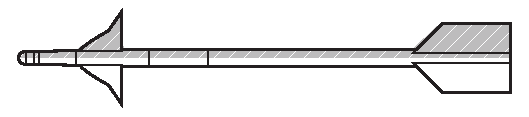
\includegraphics[
                    width = 0.8\textwidth,
            ]{diagrams/weap/weap_aa_aim9_overview.pdf}
        };

        \node[
            anchor=south west,
            font=\titlefont\huge,
        ] (aim9) at (fig.north west) {AIM-9};
        \node[
            anchor=north west,
        ] (sw) at (aim9.south west) {%
            \fontspec[
				Path=./fonts/,
				Ligatures=TeX,
				LetterSpace=5.0,
			]{Spartan MB-Regular}
            SIDEWINDER%
        };

    \end{tikzpicture}
    \caption{AIM-9 Sidewinder}
\end{figure}

\begin{tcoloritemize}
    \blueitem{AIM-9 \break Sidewinder}{
    Short-range, fire-and-forget ``dogfight'' missile. First entered service in 1956

    \begin{itemize}
        \item \textbf{Guidance} --- IR-guided (\textbf{Fox 2})
        \item \textbf{Range} --- min: \textasciitilde3000ft, max: \textasciitilde10-20nm
    \end{itemize}}
    \blueitem{Variants}{
    \begin{itemize}
        \item \textbf{9M} --- IR-guided, short range, all-aspect
        \item \textbf{9X} --- HOBS (\textbf{H}igh \textbf{O}ff-\textbf{B}ore\textbf{S}ight) capable, thrust-vectored, all-aspect
    \end{itemize}}
    \blueitem{Acquisition / Cueing Modes}{
    \begin{itemize}
        \item \textbf{Acquisition with own missile seeker (BORE)} \\
        \hyperref[subsec:aim9:bore]{See \Cref{subsec:aim9:bore}}
        \item \textbf{Seeker cued with HMD LOS (BORE)} \\
        {See \Cref{subsec:aim9:hmcs}}
        \item \textbf{Seeker slaved to radar track LOS (SLAVE)} \\
        \hyperref[subsec:aim9:slave]{See \Cref{subsec:aim9:slave}}
    \end{itemize}}
    \blueitem{Select AIM-9}{
    Via Dogfight --- AIM-9 \& GUN automatically selected

    \begin{enumerate}
        \item \textbf{DGFT/MSL OVRD} \dotfill \textbf{DGFT}
        \item \textbf{Selected Weapon (OSB 7)} \dotfill Verify \textbf{9LM / 9X}
    \end{enumerate}

    Via Missile Override

    \begin{enumerate}
        \item \textbf{DGFT/MSL OVRD} \dotfill \textbf{OVRD}
        \item \textbf{Selected Weapon (SMS OSB 7)} \dotfill \textbf{9LM / 9X}
    \end{enumerate}

    Via A-A Master Mode

    \begin{enumerate}
        \item \textbf{Master Mode} \dotfill \textbf{A-A}
        \item \textbf{Operating Mode (SMS OSB 1)} \dotfill Verify \textbf{AAM}
        \item \textbf{Selected Weapon (SMS OSB 7)} \dotfill \textbf{9LM / 9X}
    \end{enumerate}
    
    Selected weapon can also be cycled with \textbf{NWS/MSL Step depress (long)}
    }
\end{tcoloritemize}
    
\subsubsection{SMS CONTROLS}

\begin{tcoloritemize}
    \blueitem{SPOT / SCAN}{
    \textbf{OSB 2} controls seeker field of view
    \begin{itemize}
        \item \textbf{SPOT} --- Narrow, increased detection range
        \item \textbf{SCAN} --- Wide, decreased detection range
    \end{itemize}}
    \blueitem{Selected Weapon}{
    \textbf{OSB 7} cycles through available A-A weapon types
    
    \medskip
    Selected weapon can also be cycled with \textbf{NWS/MSL Step depress (long)}
    }
    \blueitem{WARM / COOL}{
    \textbf{OSB 8} controls seeker cooling status

    \begin{itemize}
        \item \textbf{COOL} ---  increases seeker sensitivity, should be set prior to engagement
        \item Set automatically for \textbf{DGFT} \& \textbf{MSL OVRD}
    \end{itemize}}
    \blueitem{Selected Station}{
    \textbf{OSB 10 / 16} select/cycle available missile pylons
    
    \medskip
    Selected station can also be cycled with \textbf{NWS/MSL Step depress (short)}
    }
    \blueitem{SLAVE / BORE}{
    \textbf{OSB 19} controls seeker line-of-sight

    \begin{itemize}
        \item \textbf{BORE} --- \hyperref[subsec:aim9:bore]{\textbf{See \Cref{subsec:aim9:bore}}}
        \begin{itemize}
            \item acquisition with own missile seeker
            \item or cued with HMD (if powered)
            \item \textbf{does NOT require FCR}
        \end{itemize}
        \item \textbf{SLAVE} --- \hyperref[subsec:aim9:slave]{\textbf{See \Cref{subsec:aim9:slave}}}
        \begin{itemize}
            \item seeker slaved to radar track LOS
            \item typically via ACM Modes
        \end{itemize}
    \end{itemize}
    
    Line-of-sight mode can also be cycled with \textbf{Cursor Enable Depress}}
\end{tcoloritemize}

\begin{figure}[htbp]
    \centering
    \begin{tikzpicture}[auto, node distance=10mm, x=1mm, y=1mm, very thick, line cap=round,
        >={Latex[round]}
        ]
        
        \node[] (fig) at (0,0) {
            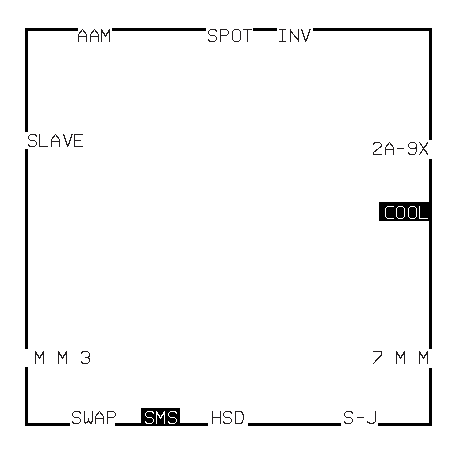
\includegraphics[
                height=75mm,
            ]{mfd/sms/aim9.pdf}
        };

        % Annotations
        \node[lannot] (mode) at ($(fig.west)+(0mm,26mm)$) {Operating \\ mode};
        \draw[annotptr] (mode.east) -- ++(12mm, 0mm) -- ++(3mm,3mm);

        \node[lannot] (los) at ($(fig.west)+(0mm,14.5mm)$) {LOS mode};
        \draw[annotptr] (los.east) -- ++(4mm, 0mm);

        \node[lannot] (lstation) at ($(fig.west)+(0mm,-21mm)$) {Selected station};
        \draw[annotptr] (lstation.east) -- ++(4mm, 0mm);

        \node[rannot] (inv) at ($(fig.east)+(0mm,26mm)$) {Inventory};
        \draw[annotptr] (inv.west) -- ++(-23mm, 0mm) -- ++(-3mm, 3mm);

        \node[rannot] (sel) at ($(fig.east)+(0mm,13mm)$) {Selected \\ weapon};
        \draw[annotptr] (sel.west) -- ++(-4mm, 0mm);

        \node[rannot] (cool) at ($(fig.east)+(0mm,3mm)$) {Cooling \\ status};
        \draw[annotptr] (cool.west) -- ++(-4mm, 0mm);

        \node[rannot] (lstation) at ($(fig.east)+(0mm,-21mm)$) {Selected station};
        \draw[annotptr] (lstation.west) -- ++(-4mm, 0mm);

        \node[rannot] (sj) at ($(fig.east)+(0mm,-36mm)$) {Selective Jettison};
        \draw[annotptr] (sj.west) -- ++(-12mm, 0mm) -- ++(-3mm, 3mm);
    \end{tikzpicture}
    \caption{AIM-9 SMS Page}
    \label{fig:aa_weap:aim9:sms}
\end{figure}

\clearpage

\subsubsection{SYMBOLOGY}
\begin{tcoloritemize}
    \blueitem{MFD Symbology}{Reference \Cref{subsec:aim120:symb}}
    \blueitem{HUD/HMD \break Symbology}{
    \begin{itemize}
        \item \textbf{Missile Diamond} --- AIM-9 seeker line-of-sight
        \begin{itemize}
            \item displayed on HUD \& HMD
            \item marked with \textbf{X} if beyond seeker limits
        \end{itemize}
        \item \textbf{Missile Reticle} --- AIM-9 seeker field-of-view
        \begin{itemize}
            \item displayed on HUD only
            \item size reflects \textbf{SPOT/SCAN} setting 
        \end{itemize}
        \item \textbf{Dynamic Aiming Cross} --- HMD line-of-sight
    \end{itemize}

    Reference symbology in \cref{fig:aa_weap:aim9:hudsymb}

    \begin{itemize}
        \item \textbf{DLZ} --- \textbf{D}ynamic \textbf{L}aunch \textbf{Z}one
        \begin{itemize}
            \item displays missile/target range information
            \item reference \Cref{subsec:aim120:symb}
        \end{itemize}
    \end{itemize}
    }
\end{tcoloritemize}

\begin{figure}[htbp]
    \centering
    \begin{tikzpicture}[auto, node distance=10mm, x=1mm, y=1mm, very thick, line cap=round,
        >={Latex[round]}
        ]
        
        \node[draw, rounded corners] (fig) at (0,0) {
            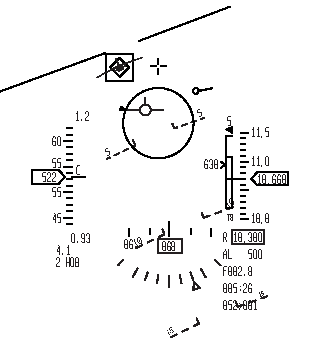
\includegraphics[
                height=75mm,
            ]{hud/aim9/full.pdf}
        };

        \node[
            draw,
            rounded 
            corners, 
            red, 
            minimum width=8.5mm, 
            minimum height=25mm
        ] (dlznode) at (12.5,1) {};

        % Annotations
        \node[lannot] (td) at ($(fig.west)+(-2.5mm,22.5mm)$) {Target designator box};
        \draw[annotptr] (td.east) -- ++(25mm, 0mm);

        \node[lannot] (diamond) at ($(fig.west)+(-2.5mm,12.5mm)$) {Missile \\ diamond};
        \draw[annotptr] (diamond.east) -- ++(18mm, 0mm) -- (-11mm, 21mm);

        \node[lannot] (weap) at ($(fig.west)+(-2.5mm,-19.5mm)$) {Selected weapon};
        \draw[annotptr] (weap.east) -- ++(15mm, 0mm);

        \node[rannot] (cross) at ($(fig.east)+(2.5mm,34mm)$) {Boresight \\ cross};
        \draw[annotptr] (cross.west) -- ++(-25mm, 0mm) -- (1mm, 24.5mm);

        \node[rannot] (ret) at ($(fig.east)+(2.5mm,24mm)$) {Missile \\ reticle};
        \draw[annotptr] (ret.west) -- ++(-30mm, 0mm) -- (4mm, 19mm);

        \node[rannot] (dlz) at ($(fig.east)+(2.5mm,-15mm)$) {DLZ};
        \draw[annotptr] (dlz.west) -- ++(-10mm, 0mm) -- (dlznode);
    \end{tikzpicture}
    \caption{AIM-9 HUD Symbology}
    \label{fig:aa_weap:aim9:hudsymb}
\end{figure}

\begin{figure}[htbp]
    \centering
    \begin{tikzpicture}[auto, node distance=10mm, x=1mm, y=1mm, very thick, line cap=round,
        >={Latex[round]}
        ]
        
        \node[draw, rounded corners] (fig) at (0,0) {
            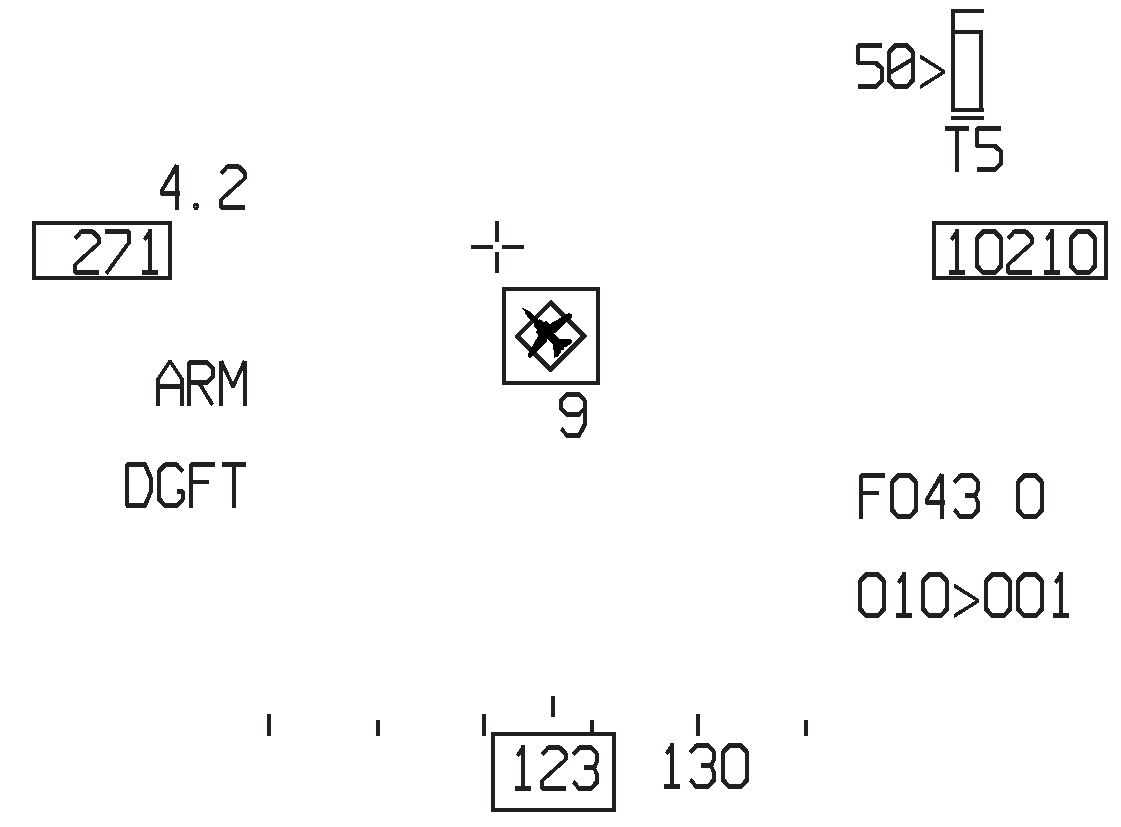
\includegraphics[
                height=50mm,
            ]{hmd/aim9_locked.pdf}
        };

        % Annotations
        \node[lannot] (diamond) at ($(fig.west)+(-2.5mm,20mm)$) {Boresight cross};
        \draw[annotptr] (diamond.east) -- ++(20mm, 0mm) -- (-5.5mm, 11.5mm);

        \node[lannot] (td) at ($(fig.west)+(-2.5mm,5mm)$) {Target designator box};
        \draw[annotptr] (td.east) -- ++(33mm, 0mm);

        \node[lannot] (mode) at ($(fig.west)+(-2.5mm,-10mm)$) {Mode};
        \draw[annotptr] (mode.east) -- ++(7.5mm, 0mm) -- (-27mm, -7mm);

        \node[rannot] (dlz) at ($(fig.east)+(2.5mm,20mm)$) {DLZ};
        \draw[annotptr] (dlz.west) -- ++(-10mm, 0mm);

        \node[rannot] (diamond) at ($(fig.east)+(2.5mm,0mm)$) {Missile \\ diamond};
        \draw[annotptr] (diamond.west) -- ++(-32mm, 0mm) -- (1.5mm, 3mm);
    \end{tikzpicture}
    \caption{AIM-9 HMD Symbology}
    \label{fig:aa_weap:aim9:hmdsymb}
\end{figure}

\marginfigeometry

\subsubsection{AIM-9 SELECTION}
\begin{checklistitemize}
    \blueitem{Via DGFT}{(AIM-9 selected automatically)
    \begin{enumerate}
        \item \textbf{DGFT/MSL OVRD} \dotfill \textbf{DGFT}
    \end{enumerate}}
    \blueitem{Via MSL OVRD}{
    \begin{enumerate}
        \item \textbf{DGFT/MSL OVRD} \dotfill \textbf{MSL OVRD}
        \item \textbf{Selected Weapon} \dotfill \textbf{9M/9X}
        \begin{itemize}
            \item \textbf{SMS OSB 7} --- \textbf{Press}
            \item or \textbf{NWS/MSL STEP} --- \textbf{Press (long)}
        \end{itemize}
    \end{enumerate}}
    \blueitem{Via A-A Master Mode}{
    \begin{enumerate}
        \item \textbf{Master Mode} \dotfill \textbf{A-A}
        \item \textbf{SMS OSB 1} \dotfill \textbf{Verify AAM} (default)
        \item \textbf{Selected Weapon} \dotfill \textbf{9M/9X}
        \begin{itemize}
            \item \textbf{SMS OSB 7} --- \textbf{Press}
            \item or \textbf{NWS/MSL STEP} --- \textbf{Press (long)}
        \end{itemize}
    \end{enumerate}}
\end{checklistitemize}

\subsubsection{BORE EMPLOYMENT --- NO RADAR}
\label{subsec:aim9:bore}
\begin{checklistenumerate}
    \blueitem{Prerequisites}{
    \begin{itemize}
        \item \textbf{RF Switch} \dotfill \textbf{SILENT} \\
        \hfill (if desired, completely silences radar)
        \item \textbf{Selected Weapon} \dotfill \textbf{9M/9X}
        \item \textbf{SLAVE/BORE} \dotfill \textbf{BORE}
        \item \textbf{WARM/COOL} \dotfill Verify \textbf{COOL}
        \item \textbf{Master Arm} \dotfill \textbf{ARM}
    \end{itemize}}
    \blueitem{AIM-9 Track Acquisition}{
    \marginpar{
        \captionsetup{type=figure}
        \centering
        \begin{tikzpicture}[figstyle]
            \node[boxedmarfigstyle] (fig) at (0,0) {
                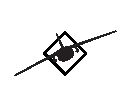
\includegraphics[
                    scale=1.25,
                ]{hud/aim9/subfig_missile_diamond.pdf}
            };
        \end{tikzpicture}
        \caption{AIM-9 missile diamond latched to target, indicating lock.}
    }
    \begin{enumerate}
        \item \textbf{Missile Reticle} \dotfill \textbf{On-Target}
        \item \textbf{Sidewinder Audio} \dotfill \textbf{Lock Tone}
        \item \textbf{CAGE/UNCAGE} \dotfill \textbf{Press}
        \item \textbf{Missile Diamond} \dotfill verify latched to target
    \end{enumerate}}
    \blueitem{Fire Missile}{
    \begin{enumerate}
        \item Maneuver into firing position
        \item \textbf{Sidewinder Audio} \dotfill \textbf{Lock Tone}
        \item \textbf{WPN REL} \dotfill \textbf{Depress}
    \end{enumerate}}
\end{checklistenumerate}

\clearpage

\subsubsection{HMCS BORE EMPLOYMENT --- NO RADAR}
\label{subsec:aim9:hmcs}
\begin{checklistenumerate}
    \blueitem{Prerequisites}{
    \begin{itemize}
        \item \textbf{HMD SYMB. INT} \dotfill \textbf{INT}
        \item \textbf{RF Switch} \dotfill \textbf{SILENT} \\
        \hfill (if desired, completely silences radar)
        \item \textbf{Selected Weapon} \dotfill \textbf{9M/9X}
        \item \textbf{SLAVE/BORE} \dotfill \textbf{BORE}
        \item \textbf{WARM/COOL} \dotfill Verify \textbf{COOL}
        \item \textbf{Master Arm} \dotfill \textbf{ARM}
    \end{itemize}}
    \blueitem{AIM-9 Track Acquisition}{
    \marginpar{
        \captionsetup{type=figure}
        \begin{tikzpicture}[figstyle]
            \node[boxedmarfigstyle] (fig) at (0,0) {
                
\includegraphics[
                    scale=0.75,
                ]{hmd/aiming_cross.pdf}
            };
        \end{tikzpicture}
        \caption{AIM-9 seeker follows HMD aiming cross}
    }
    \marginpar{
        \captionsetup{type=figure}
        \begin{tikzpicture}[figstyle]
            \node[boxedmarfigstyle] (fig) at (0,0) {
                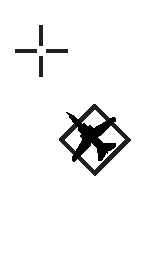
\includegraphics[
                    scale=0.5,
                ]{hmd/aim9_track_missile_diamond.pdf}
            };
        \end{tikzpicture}
        \caption{AIM-9 HMD track}
    }
    \marginpar{
        \captionsetup{type=figure}
        \begin{tikzpicture}[figstyle]
            \node[boxedmarfigstyle] (fig) at (0,0) {
                
\includegraphics[
                    scale=0.75,
                ]{hmd/los.pdf}
            };
        \end{tikzpicture}
        \caption{X indicates HMD beyond AIM-9 seeker limits}
    }
    \begin{enumerate}
        \item Maneuver to place target within AIM-9 seeker limits
        \item \textbf{HMD Aiming Cross} \dotfill \textbf{On-Target}
    \end{enumerate}

    Missile diamond follows aiming cross (within seeker limits)

    \begin{enumerate}[start=3]
        \item \textbf{Sidewinder Audio} \dotfill \textbf{Lock Tone}
        \item \textbf{CAGE/UNCAGE} \dotfill \textbf{Press}
        \item \textbf{Missile Diamond} \dotfill verify latched to target
    \end{enumerate}}
    \blueitem{Fire Missile}{
    \begin{enumerate}
        \item Maneuver into firing position
        \item \textbf{Sidewinder Audio} \dotfill \textbf{Lock Tone}
        \item \textbf{WPN REL} \dotfill \textbf{Depress}
    \end{enumerate}}
\end{checklistenumerate}

\clearpage

\subsubsection{SLAVE EMPLOYMENT --- RADAR}
\label{subsec:aim9:slave}
\begin{checklistenumerate}
    \blueitem{Prerequisites}{
    \begin{itemize}
        \item \textbf{FCR Switch} \dotfill \textbf{FCR}
        \item \textbf{RF Switch} \dotfill \textbf{NORM}
        \item \textbf{HMD SYMB. INT} \dotfill As desired
        \item \textbf{Selected Weapon} \dotfill \textbf{9M/9X}
        \item \textbf{SLAVE/BORE} \dotfill Verify \textbf{SLAVE}
        \item \textbf{WARM/COOL} \dotfill Verify \textbf{COOL}
        \item \textbf{Master Arm} \dotfill \textbf{ARM}
    \end{itemize}}
    \blueitem{Radar Acquisition}{ACM selected automatically in \textbf{DGFT} mode, \textbf{see \Cref{subsec:acm}}
    \marginpar{
        \captionsetup{type=figure}
        \centering
        \begin{tikzpicture}[figstyle]

            % \draw[color2, fill=color2!20, dashed] 
            % (0,-6) circle [x radius=8, y radius=11.5];
            
            \node[boxedmarfigstyle] (bore) at (0,0) {
                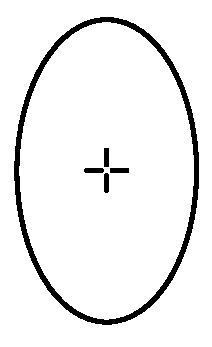
\includegraphics[
                    scale=0.5,
                ]{hmd/dgft_subfig_bore.pdf}
            };
        \end{tikzpicture}
        \caption{HMD BORE scan zone}
    }
    
    \medskip
    For demonstration we will use \textbf{ACM BORE Submode} with HMD
    
    \begin{enumerate}
        \item \textbf{FCR Mode} \dotfill \textbf{ACM}
        \item \textbf{TMS} \dotfill \textbf{FWD}
        \item \textbf{Target} \dotfill \textbf{In HMD BORE Symbol}
        \item \textbf{Radar} \dotfill wait for \textbf{STT Lock}
    \end{enumerate}
    
    Can also lock from CRM, \textbf{see \Cref{subsec:crm}}
    }
    \blueitem{AIM-9 Track Acquisition}{
    \marginpar{
        \captionsetup{type=figure}
        \centering
        \begin{tikzpicture}[figstyle]
            \node[boxedmarfigstyle] (fig) at (0,0) {
                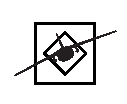
\includegraphics[
                    scale=1.25,
                ]{hud/aim9/subfig_td_box_missile_diamond.pdf}
            };
        \end{tikzpicture}
        \caption{AIM-9 missile diamond and target designator box latched to target, indicating radar and seeker lock.}
    }
    \begin{enumerate}
        \item \textbf{CAGE/UNCAGE} \dotfill \textbf{Press}
        \item \textbf{Sidewinder Audio} \dotfill \textbf{Lock Tone}
        \item \textbf{Missile Diamond} \dotfill verify latched to target
    \end{enumerate}}
    \blueitem{Fire Missile}{
    \marginpar{
        \captionsetup{type=figure}
        \centering
        \begin{tikzpicture}[figstyle]
            \node[boxedmarfigstyle] (fig) at (0,0) {
                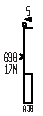
\includegraphics[
                    scale=2.5,
                ]{hud/aim9/subfig_dlz.pdf}
            };
        \end{tikzpicture}
        \caption{In-range DLZ}
    }
    \begin{enumerate}
        \item Maneuver into firing position
        \item \textbf{DLZ} \dotfill indicates \textbf{In-Range}
        \item \textbf{Sidewinder Audio} \dotfill \textbf{Lock Tone}
        \item \textbf{WPN REL} \dotfill \textbf{Depress}
    \end{enumerate}}
\end{checklistenumerate}

\marginfigrestore 

\subsection{AIM-120 AMRAAM}
\label{subsec:aim120}
\begin{figure}[htbp]
    \centering
    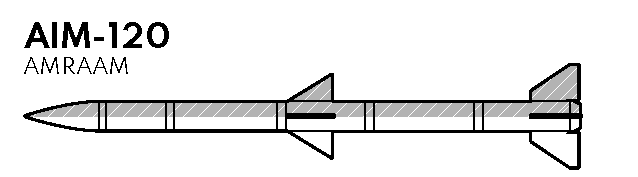
\includegraphics[
            width = 108mm,
    ]{diagrams/weap/weap_aa_amraam_overview.pdf}
    % TODO: flavor text/stuff?
    \caption{AIM-120 AMRAAM}
\end{figure}

\begin{tcoloritemize}
    \blueitem[AIM-120 \break AMRAAM]
    \textbf{A}dvanced \textbf{M}edium \textbf{R}ange \textbf{A}ir-to-\textbf{A}ir \textbf{M}issile
    --- long range, fire-and-forget, active-radar homing missile

    \begin{itemize}
        \item \textbf{Guidance} --- Active Radar-Guided (\textbf{Fox 3})
        \item \textbf{Range} --- max:  \textasciitilde30-40nm (high mach, alt)
    \end{itemize}
    \blueitem[Employment \break Types]
    \begin{itemize}
        \item \textbf{Maddog / Active Launch  (no radar)} \\
        \hyperref[subsec:aim120:maddog]{see \Cref{subsec:aim120:maddog}}
        \item \textbf{Single-target employment (STT lock or TWS/DTT bug)}
        \hyperref[subsec:aim120:single]{see \Cref{subsec:aim120:single}}
        \item \textbf{Multi-target employment (TWS/DTT bug)} \\
        \hyperref[subsec:aim120:multi]{see \Cref{subsec:aim120:multi}}
    \end{itemize}
    \blueitem[Flight Profile]
    Successful long-range weapon employment necessitates understanding of flight-profile and tactics
    \begin{itemize}
        \item \textbf{Mid-Course} --- Guided via \underline{datalink}, launching fighter should maintain radar contact with target
        \item \textbf{Terminal Phase} --- Guided via \underline{internal radar}, launching fighter may break away
    \end{itemize}
    
    \textbf{See \Cref{subsec:bvr} and \Cref{subsec:bvr:rangeconsideration}}
    \blueitem[Select AIM-120]
    Via A-A Master Mode

    \begin{enumerate}
        \item \textbf{Master Mode} \dotfill \textbf{A-A}
        \item \textbf{Operating Mode (SMS OSB 1)} \dotfill Verify \textbf{AAM}
        \item \textbf{Selected Weapon (SMS OSB 7)} \dotfill \textbf{120C}
    \end{enumerate}

    Via Missile Override

    \begin{enumerate}
        \item \textbf{DGFT/MSL OVRD} \dotfill \textbf{OVRD}
        \item \textbf{Selected Weapon (SMS OSB 7)} \dotfill \textbf{120C} 
    \end{enumerate}
    
    Via Dogfight

    \begin{enumerate}
        \item \textbf{DGFT/MSL OVRD} \dotfill \textbf{DGFT}
        \item \textbf{Selected Weapon (SMS OSB 7)} \dotfill \textbf{120C}
    \end{enumerate}
    
    Selected weapon can also be cycled with \textbf{NWS/MSL Step depress (long)}
\end{tcoloritemize}

\subsubsection{SMS CONTROLS}
\label{subsec:aim120:sms}
\begin{tcoloritemize}
    \blueitem[Selected Weapon]
    \textbf{OSB 7} cycles through available A-A weapon types
    
    \medskip
    Selected weapon can also be cycled with \textbf{NWS/MSL Step depress (long)}
    \blueitem[Selected Station]
    \textbf{OSB 10 / 16} select/cycle availabel missile pylons
    
    \medskip
    Selected station can also be cycled with \textbf{NWS/MSL Step depress (short)}
    \blueitem[SLAVE / BORE]
    \textbf{OSB 19} controls missile radar line-of-sight
    \begin{itemize}
        \item \textbf{SLAVE} --- Missile LOS slaved to AC radar 
        \begin{itemize}
            \item receives DL updates until within own radar limits
        \end{itemize}
        \item \textbf{BORE} --- Missile scans straight ahead
        \begin{itemize}
            \item tracks first detected target
        \end{itemize}
    \end{itemize}
    
    Line-of-sight mode can also be cycled with \textbf{Cursor Enable Depress}
\end{tcoloritemize}

\begin{figure}[htbp]
    \centering
    \begin{tikzpicture}[auto, node distance=10mm, x=1mm, y=1mm, very thick, line cap=round,
        >={Latex[round]}
        ]
        
        \node[] (fig) at (0,0) {
            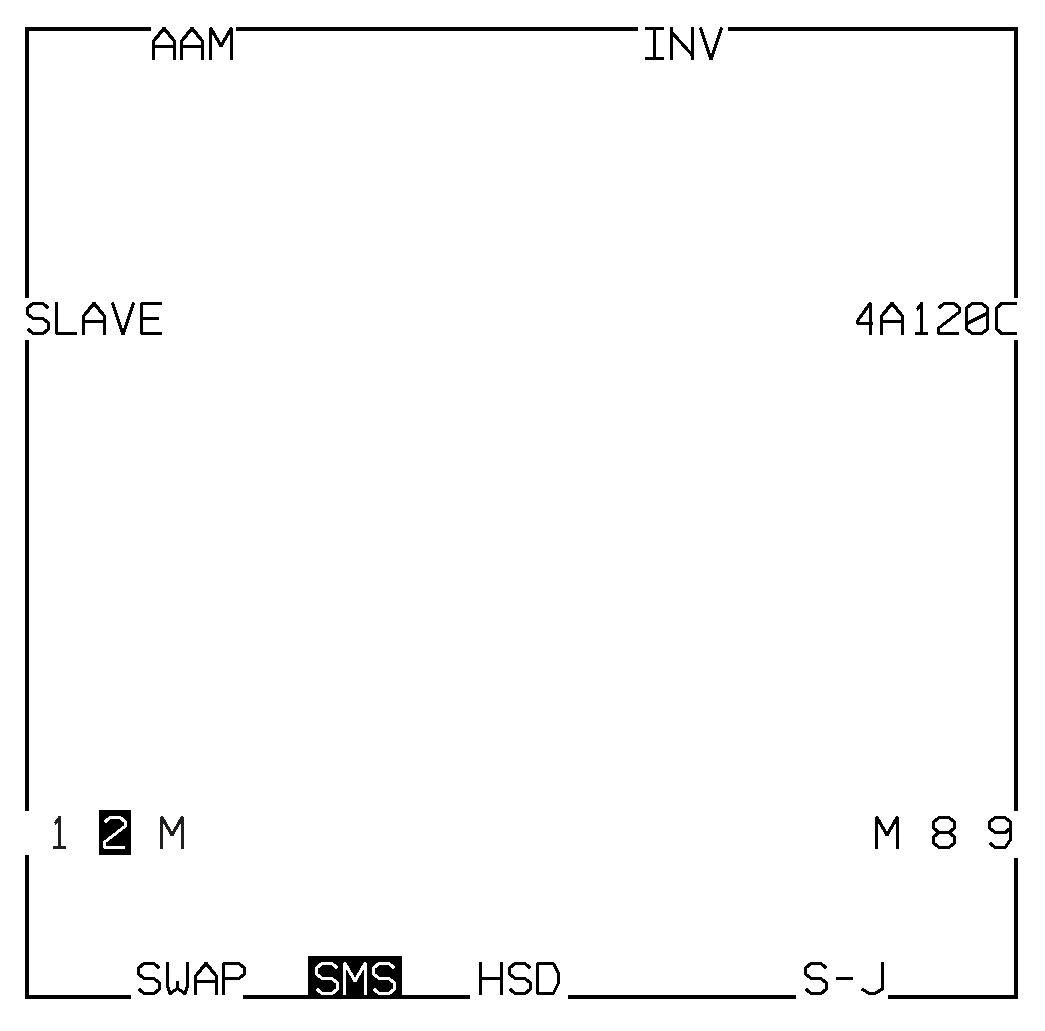
\includegraphics[
                height=75mm,
            ]{mfd/sms/aim120.pdf}
        };

        % Annotations
        \node[lannot] (mode) at ($(fig.west)+(-2.5mm,27mm)$) {Operating \\ mode};
        \draw[annotptr] (mode.east) -- ++(12mm, 0mm) -- ++(5mm,5mm);

        \node[lannot] (los) at ($(fig.west)+(-2.5mm,14.25mm)$) {LOS mode};
        \draw[annotptr] (los.east) -- ++(5mm, 0mm);

        \node[lannot] (lstation) at ($(fig.west)+(-2.5mm,-23mm)$) {Selected station};
        \draw[annotptr] (lstation.east) -- ++(5mm, 0mm);

        \node[rannot] (inv) at ($(fig.east)+(2.5mm,27mm)$) {Inventory};
        \draw[annotptr] (inv.west) -- ++(-24mm, 0mm) -- ++(-5mm, 5mm);

        \node[rannot] (sel) at ($(fig.east)+(2.5mm,14.25mm)$) {Selected \\ weapon};
        \draw[annotptr] (sel.west) -- ++(-5mm, 0mm);

        \node[rannot] (lstation) at ($(fig.east)+(2.5mm,-23mm)$) {Selected station};
        \draw[annotptr] (lstation.west) -- ++(-5mm, 0mm);

        \node[rannot] (sj) at ($(fig.east)+(2.5mm,-40mm)$) {Selective Jettison};
        \draw[annotptr] (sj.west) -- ++(-14mm, 0mm) -- ++(-4mm,4mm);
    \end{tikzpicture}
    \caption{AIM-120 SMS page}
\end{figure}

\clearpage

\subsubsection{SYMBOLOGY}
\label{subsec:aim120:symb}

\begin{tcoloritemize}
    \blueitem[Basic Radar Symbology] 
    For beyond-visual-range radar usage and symbology \textbf{reference \Crefrange{subsec:crm}{subsec:tws}}
    \blueitem[DLZ]
    \textbf{D}ynamic \textbf{L}aunch \textbf{Z}one
    \begin{itemize}
        \item \textbf{Displays target range \& missile performance information on HUD \& FCR Page with}
        \begin{itemize}
            \item missile selected
            \item radar track acquired
        \end{itemize}
        \item \textbf{R\textsubscript{aero} --- Aerodynamic range}
        \begin{itemize}
            \item \underline{maximum kinetic range}
            \item assumes non-maneuvering target
        \end{itemize}
        \item \textbf{R\textsubscript{opt} --- Optimal}
        \item \textbf{R\textsubscript{PI} --- Probability Intercept}
        \item \textbf{R\textsubscript{TR} --- Turn-and-run range}
        \begin{itemize}
            \item maximum range assuming target turns cold at current velocity
        \end{itemize}
        \item \textbf{R\textsubscript{ACT} --- Active range}
        \begin{itemize}
            \item range at which AIM-120 will go active
            \item not shown in \ref{fig:aa_weap:aim120:dlz}
        \end{itemize}
        \item \textbf{R\textsubscript{MIN} --- Minimum range}
        \item \textbf{Countdown}
        \begin{itemize}
            \item \textbf{A} --- seconds until missile goes active
            \item \textbf{T} --- seconds until predicted impact
        \end{itemize}
    \end{itemize}
    Reference \cref{fig:aa_weap:aim120:dlz}
    \blueitem[ASC \& ASEC]
    \begin{itemize}
        \item \textbf{Displays target lead cues to maximize missile performance on HUD \& FCR Page with}
        \begin{itemize}
            \item AIM-120 selected
            \item radar track acquired
        \end{itemize}
        \item \textbf{Pilot should place ASC inside ASEC}
        \item \textbf{ASC} --- \textbf{A}ttack \textbf{S}teering \textbf{C}ue
        \item \textbf{ASEC} --- \textbf{A}llowable \textbf{S}teering \textbf{E}rror \textbf{C}ircle
        \begin{itemize}
            \item dynamically adjusts size based on target maneuvers
            \item fixed size prior to target designation
        \end{itemize}
    \end{itemize}
\end{tcoloritemize}

% \clearpage

\begin{figure}[htbp]
    \centering
    \begin{subfigure}[b]{0.6\linewidth}
        \centering
        \begin{tikzpicture}[figstyle]

            \node[draw, rounded corners] (fig) at (0,0) {
                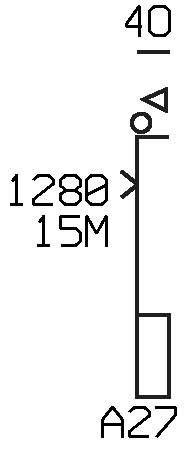
\includegraphics[
                    scale=0.5,
                ]{mfd/fcr_aa/aim120_subfig_dlz_prelaunch.pdf}
            };

            % Annotations
            \node[lannot] (rscale) at ($(fig.west)+(-2.5mm,17mm)$) {Range scale};
            \draw[annotptr] (rscale.east) -- ++(12mm, 0mm);

            \node[lannot] (tgt) at ($(fig.west)+(-2.5mm,10mm)$) {Target range};
            \draw[annotptr] (tgt.east) -- ++(8mm,0mm) -- (1.5mm, 6mm);

            \node[lannot] (closure) at ($(fig.west)+(-2.5mm,3.0mm)$) {Closure};
            \draw[annotptr] (closure.east) -- ++(4mm,0mm);

            \node[lannot] (mpole) at ($(fig.west)+(-2.5mm,-6mm)$) {M-Pole};
            \draw[annotptr] (mpole.east) -- ++(6mm,0mm) -- ++(2mm, 3mm);

            \node[lannot] (apole) at ($(fig.west)+(-2.5mm,-17mm)$) {A-Pole};
            \draw[annotptr] (apole.east) -- ++(11mm,0mm);

            \node[rannot] (raero) at ($(fig.east)+(2.5mm,13mm)$) {R\textsubscript{aero}};
            \draw[annotptr] (raero.west) -- ++(-2.5mm, 0mm) -- ++(-2.5mm, -1.5mm);

            \node[rannot] (ropt) at ($(fig.east)+(2.5mm,8.5mm)$) {R\textsubscript{opt}};
            \draw[annotptr] (ropt.west) -- ++(-6mm, 0mm);

            \node[rannot] (rpi) at ($(fig.east)+(2.5mm,4mm)$) {R\textsubscript{PI}};
            \draw[annotptr] (rpi.west) -- ++(-4mm, 0mm) -- ++(-2mm, 3mm);

            \node[rannot] (rtr) at ($(fig.east)+(2.5mm,-7.5mm)$) {R\textsubscript{TR}};
            \draw[annotptr] (rtr.west) -- ++(-4mm, 0mm);

            \node[rannot] (rmin) at ($(fig.east)+(2.5mm,-14.5mm)$) {R\textsubscript{min}};
            \draw[annotptr] (rmin.west) -- ++(-4mm, 0mm);
        \end{tikzpicture}
        \caption{pre-launch}
        \label{fig:aa_weap:aim120:dlz:pre}
    \end{subfigure}

    \vspace{1em}
    \begin{subfigure}[b]{0.45\linewidth}
        \centering
        \begin{tikzpicture}[figstyle]

            \node[draw, rounded corners] (fig) at (0,0) {
                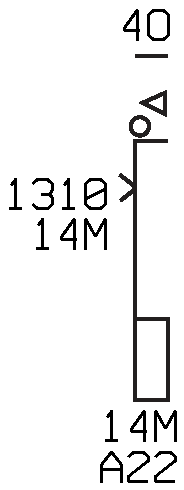
\includegraphics[
                    scale=0.5,
                ]{mfd/fcr_aa/aim120_subfig_dlz_postlaunch.pdf}
            };

            % Annotations
            \node[lannot] (mpole) at ($(fig.west)+(-2.5mm,0.75mm)$) {M-Pole \\ {\footnotesize (next)}};
            \draw[annotptr] (mpole.east) -- ++(6mm,0mm);

            \node[lannot] (mpleif) at ($(fig.west)+(-2.5mm,-10mm)$) {M-Pole \\ {\footnotesize (in-flight)}};
            \draw[annotptr] (mpleif.east) -- ++(6mm,0mm) -- ++(5.5mm, -3.5mm);

            \node[lannot, text width=30mm] (apole) at ($(fig.west)+(-2.5mm,-19mm)$) {Time-to-active \\ {\footnotesize (in-flight)}};
            \draw[annotptr] (apole.east) -- ++(11mm,0mm);
        \end{tikzpicture}
        \caption{post-launch}
        \label{fig:aa_weap:aim120:dlz:post}
    \end{subfigure}
    \begin{subfigure}[b]{0.45\linewidth}
        \centering
        \begin{tikzpicture}[figstyle]

            \node[draw, rounded corners] (fig) at (0,0) {
                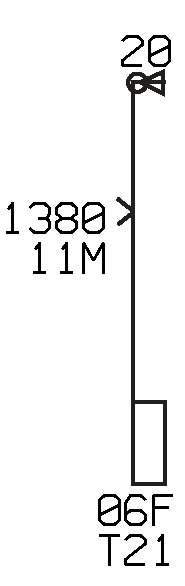
\includegraphics[
                    scale=0.5,
                ]{mfd/fcr_aa/aim120_subfig_dlz_active.pdf}
            };

            % Annotations
            \node[rannot] (fpole) at ($(fig.east)+(2.5mm,-13mm)$) {F-Pole \\ {\footnotesize (in-flight)}};
            \draw[annotptr] (fpole.west) -- ++(-2mm,0mm) -- ++(-2.5mm, -3mm);

            \node[rannot, text width=30mm] (ttg) at ($(fig.east)+(2.5mm,-22mm)$) {Time-to-impact \\ {\footnotesize (in-flight)}};
            \draw[annotptr] (ttg.west) -- ++(-4mm,0mm);
        \end{tikzpicture}
        \caption{post-active}
        \label{fig:aa_weap:aim120:dlz:act}
    \end{subfigure}
    \caption{DLZ symbology both before (a) and after (b) AIM-120 launch as well as post missile going active (c).} 
    \label{fig:aa_weap:aim120:dlz}
\end{figure}

\begin{figure}[htbp]
    \centering
    \begin{tikzpicture}[auto, node distance=10mm, x=1mm, y=1mm, very thick, line cap=round,
        >={Latex[round]}
        ]

        \node[draw, rounded corners] (fig) at (0,0) {
            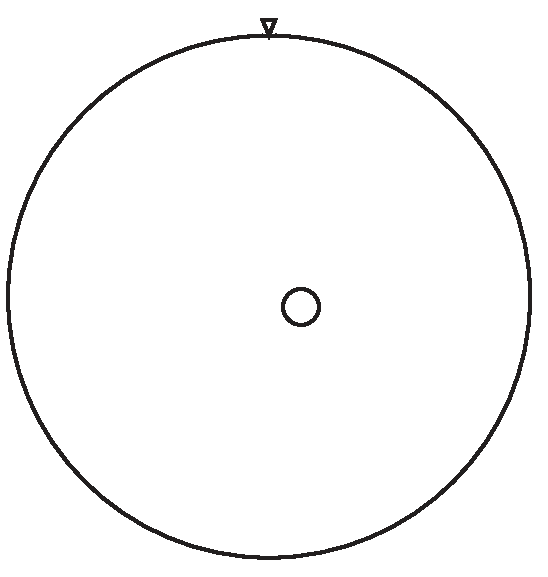
\includegraphics[
                scale=0.5,
            ]{hud/aim120/subfig_asec_asc.pdf}
        };

        % Annotations
        \node[lannot] (asec) at ($(fig.west)+(-2.5mm,20mm)$) {ASEC};
        \draw[annotptr] (asec.east) -- ++(8mm,0mm) -- ++(3mm,-3mm);

        \node[lannot] (asc) at ($(fig.west)+(-2.5mm,-10mm)$) {ASC};
        \draw[annotptr] (asc.east) -- ++(21mm,0mm) -- ++(6mm, 6mm);

        \node[rannot] (aspect) at ($(fig.east)+(2.5mm,12mm)$) {Aspect caret};
        \draw[annotptr] (aspect.west) -- ++(-18mm, 0mm) -- ++(-8mm,8mm);
    \end{tikzpicture}
    \caption{
        AIM-120 ASC / ASEC HUD symbology, equivalent symbology appears on FCR page. 
        ASC should be placed within ASEC to maximize P\textsubscript{kill}.
    }
    \label{fig:aa_weap:aim120:asc_asec}
\end{figure}

\begin{tcoloritemize}
    \blueitem[Designator Box] Box around target when within HUD view
    \blueitem[TLL]
    \textbf{T}arget \textbf{L}ocator \textbf{L}ine
    
    \begin{itemize}
        \item \textbf{Extends from boresight cross towards target}
        \item \textbf{Relative angle displayed next to boresight cross}
        \item \textbf{Displayed when target is not within HUD field-of-view}
    \end{itemize}
    \blueitem[Missile Diamond] Indicates missile seeker line-of-sight
    \blueitem[Post-Launch Symbology]
    Bugged track symbology is modified to reflect missile launch \& status

    \begin{itemize}
        \item \textbf{Post-launch} --- Thick ``tail'' is added
        \item \textbf{Post-active} --- Tail begins to flash
        \item \textbf{Post predicted impact} --- Red cross flashes over track
    \end{itemize}
\end{tcoloritemize}

\begin{figure}[htbp]
    \centering
    \begin{tikzpicture}[auto, node distance=10mm, x=1mm, y=1mm, very thick, line cap=round,
        >={Latex[round]}
        ]
        \node[draw, rounded corners] (fig) at (0,0) {
            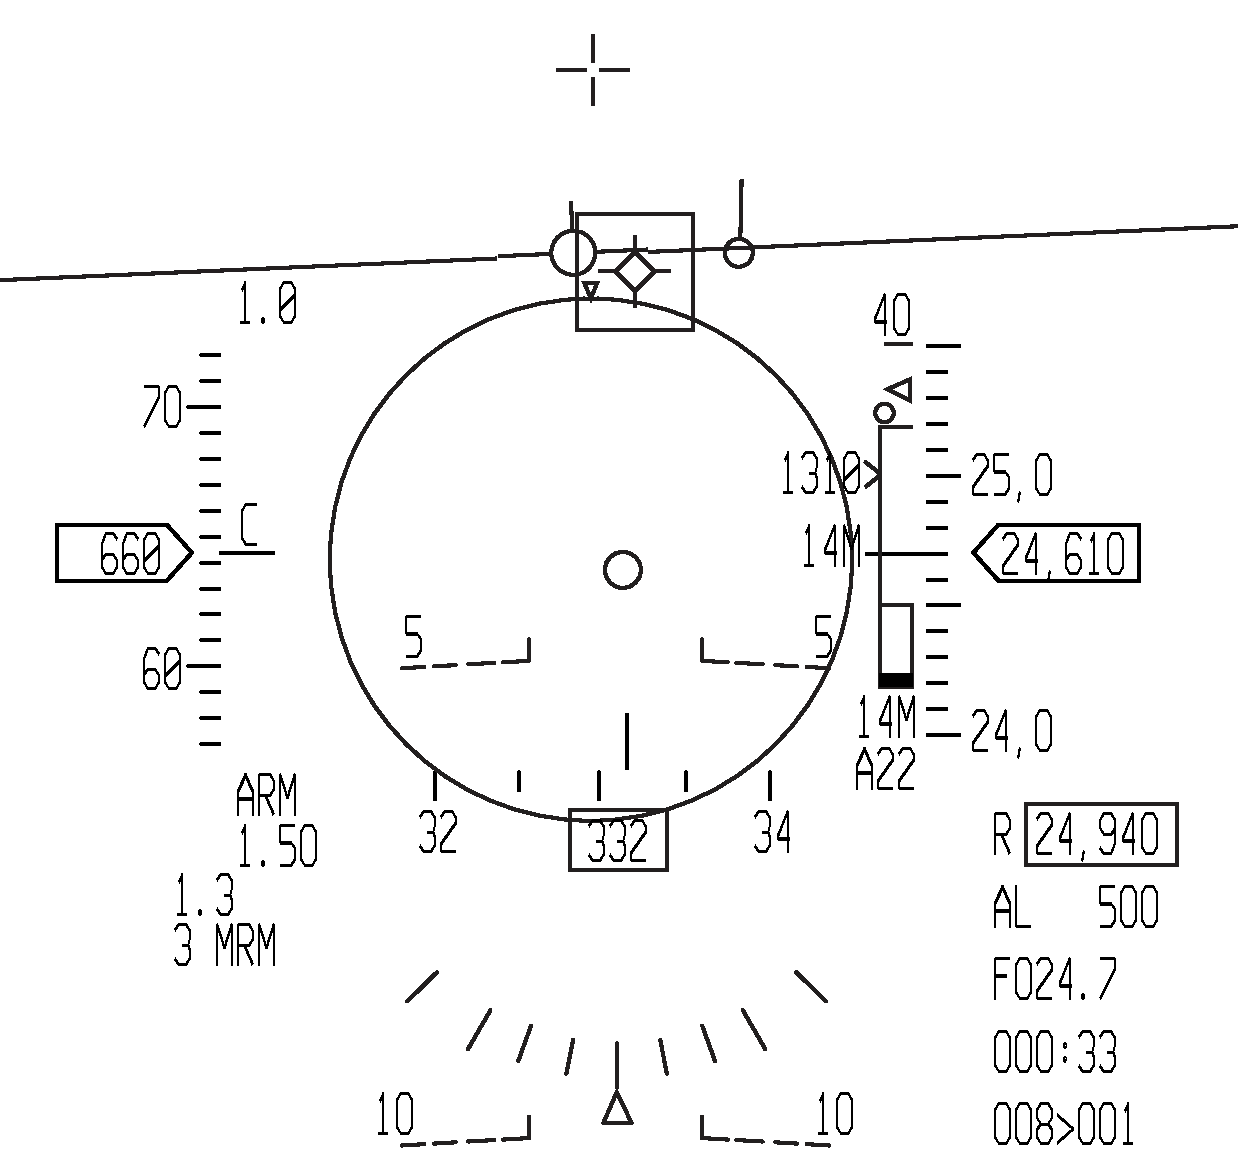
\includegraphics[
                height=75mm,
            ]{hud/aim120/postlaunch.pdf}
        };

        \node[
            draw,
            rounded 
            corners, 
            red, 
            minimum width=10.5mm, 
            minimum height=34mm
        ] (dlznode) at (14.5,3) {};

        % Annotations
        \node[lannot] (td) at ($(fig.west)+(-2.5mm,30mm)$) {Target designator box};
        \draw[annotptr] (td.east) -- ++(40mm, 0mm) -- (0mm, 25mm);

        \node[lannot] (asec) at ($(fig.west)+(-2.5mm,9mm)$) {ASC \\ {\footnotesize see \cref{fig:aa_weap:aim120:asc_asec}}};
        \draw[annotptr] (asec.east) -- ++(30mm, 0mm) -- (-2mm, 2mm);

        \node[lannot] (asec) at ($(fig.west)+(-2.5mm,-9.5mm)$) {ASEC \\ {\footnotesize see \cref{fig:aa_weap:aim120:asc_asec}}};
        \draw[annotptr] (asec.east) -- ++(20mm, 0mm) -- (-18mm, -6mm);

        \node[lannot] (weap) at ($(fig.west)+(-2.5mm,-23mm)$) {Selected weapon};
        \draw[annotptr] (weap.east) -- ++(14mm, 0mm);

        \node[rannot] (diamond) at ($(fig.east)+(2.5mm,30mm)$) {Missile \\ diamond};
        \draw[annotptr] (diamond.west) -- ++(-25mm, 0mm) -- (2.5mm, 21mm);

        \node[rannot] (dlz) at ($(fig.east)+(2.5mm,-5mm)$) {DLZ \\ {\footnotesize see \cref{fig:aa_weap:aim120:dlz}}};
        \draw[annotptr] (dlz.west) -- ++(-10mm, 0mm) -- (dlznode);

        \node[rannot] (range) at ($(fig.east)+(2.5mm,-25.5mm)$) {Target range};
        \draw[annotptr] (range.west) -- ++(-11mm, 0mm);
    \end{tikzpicture}
    \caption{AIM-120 HUD symbology post-launch}
\end{figure}

\begin{figure}[htbp]
    \centering
    \begin{tikzpicture}[auto, node distance=10mm, x=1mm, y=1mm, very thick, line cap=round,
        >={Latex[round]}
        ]
        
        \node[] (fig) at (0,0) {
            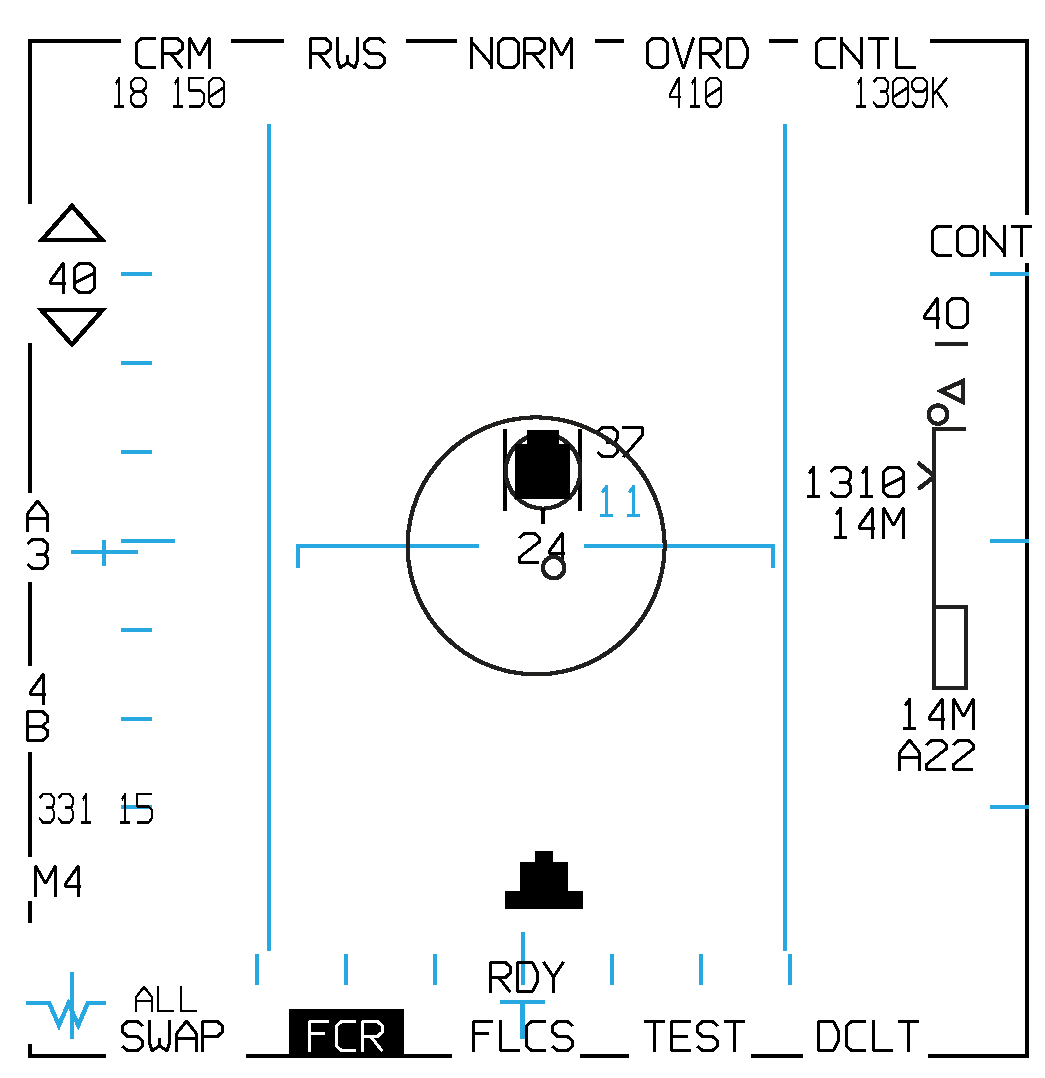
\includegraphics[
                height=75mm,
            ]{mfd/fcr_aa/aim120_postlaunch.pdf}
        };

        % Annotations
        \node[lannot] (aspect) at ($(fig.west)+(-2.5mm, 31mm)$) {Aspect};
        \draw[annotptr] (aspect.east) -- ++(11mm, 0mm);

        \node[lannot] (track) at ($(fig.west)+(-2.5mm, 24.5mm)$) {Ground track};
        \draw[annotptr] (track.east) -- ++(14mm, 0mm) -- (-23mm,29mm);

        \node[lannot] (tgt) at ($(fig.west)+(-2.5mm,10mm)$) {Target \\ {\footnotesize with tail}};
        \draw[annotptr] (tgt.east) -- ++(25mm, 0mm) -- (-2mm, 5mm);

        \node[lannot] (asec) at ($(fig.west)+(-2.5mm,-5mm)$) {ASEC / ASC \\ {\footnotesize see \cref{fig:aa_weap:aim120:asc_asec}}};
        \draw[annotptr] (asec.east) -- ++(30mm, 0mm) -- (-8mm, -4mm);

        \node[lannot] (bulls) at ($(fig.west)+(-2.5mm,-18.5mm)$) {Bullseye of cursor};
        \draw[annotptr] (bulls.east) -- ++(5mm, 0mm);

        \node[rannot] (closure) at ($(fig.east)+(2.5mm,31mm)$) {Closure};
        \draw[annotptr] (closure.west) -- ++(-10mm, 0mm);

        \node[rannot] (as) at ($(fig.east)+(2.5mm,25mm)$) {Airspeed};
        \draw[annotptr] (as.west) -- ++(-24mm, 0mm) -- (14mm, 29mm);

        \node[rannot] (dlz) at ($(fig.east)+(2.5mm,0mm)$) {DLZ \\ {\footnotesize see \cref{fig:aa_weap:aim120:dlz}}};
        \draw[annotptr] (dlz.west) -- ++(-8mm, 0mm);
    \end{tikzpicture}
    \caption{AIM-120 FCR page post-launch. Note the ``tail'' on the track. Tail flashes once AIM-120 has gone active.}
\end{figure}

\begin{figure}[htbp]
    \centering
    \begin{subfigure}[t]{0.3\linewidth}
        \centering
        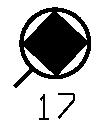
\includegraphics[
            scale=0.75,
        ]{mfd/fcr_aa/tgt_bugged.pdf}
        \caption{bugged target}
    \end{subfigure}
    \begin{subfigure}[t]{0.3\linewidth}
        \centering
        
\includegraphics[
            scale=0.75,
        ]{mfd/fcr_aa/tgt_tail.pdf}
        \caption{indicates AIM-120 launched}
    \end{subfigure}
    \begin{subfigure}[t]{0.3\linewidth}
        \centering
        
\includegraphics[
            scale=0.75,
        ]{mfd/fcr_aa/tgt_impact.pdf}
        \caption{indicates predicted t\textsubscript{imp} has occured}
    \end{subfigure}
    \caption{
        FCR page target symbology relating to AIM-120. 
        ``Tail'' appears once AIM-120 has been launched and flashes once missile has gone active. 
        Red ``X'' indicates missile time-of-impact has occured.
    }
\end{figure}

\marginfigeometry

\subsubsection{AIM-120 SELECTION}
\label{subsec:aim120:selection}
\begin{checklistitemize}
    \blueitem[Via A-A Master Mode]
    \begin{enumerate}
        \item \textbf{Master Mode} \dotfill \textbf{A-A}
        \item \textbf{SMS OSB 1} \dotfill Verify \textbf{AAM}
        \item \textbf{Selected Weapon} \dotfill Verify \textbf{120C}
        \begin{itemize}
            \item \textbf{SMS OSB 7} --- \textbf{Press}
            \item or \textbf{NWS/MSL STEP} --- \textbf{Press (long)}
        \end{itemize}
    \end{enumerate}
    \blueitem[Via MSL OVRD]
    \begin{enumerate}
        \item \textbf{DGFT/MSL OVRD} \dotfill \textbf{OVRD}
        \item \textbf{Selected Weapon} \dotfill Verify \textbf{120C} 
        \begin{itemize}
            \item \textbf{SMS OSB 7} --- \textbf{Press}
            \item or \textbf{NWS/MSL STEP} --- \textbf{Press (long)}
        \end{itemize}
    \end{enumerate}
    \blueitem[Via DGFT]
    \begin{enumerate}
        \item \textbf{DGFT/MSL OVRD} \dotfill \textbf{DGFT}
        \item \textbf{Selected Weapon} \dotfill \textbf{120C}
        \begin{itemize}
            \item \textbf{SMS OSB 7} --- \textbf{Press}
            \item or \textbf{NWS/MSL STEP} --- \textbf{Press (long)}
        \end{itemize}
    \end{enumerate}
\end{checklistitemize}

\subsubsection{MADDOG EMPLOYMENT --- NO RADAR}
\label{subsec:aim120:maddog}
\begin{checklistenumerate}
    \blueitem[Prerequisites]
    \begin{itemize}
        \item \textbf{RF Switch} \dotfill \textbf{SILENT} \\
        \hfill (if desired, completely silences radar)
        \item \textbf{Selected Weapon} \dotfill \textbf{120C}
        \item \textbf{SLAVE/BORE} \dotfill \textbf{BORE}
        \begin{itemize}
            \item \textbf{SMS OSB 19} --- \textbf{Press}
            \item or \textbf{Cursor Enable} --- \textbf{Press}
        \end{itemize}
        \item \textbf{Master Arm} \dotfill \textbf{ARM}
    \end{itemize}
    \blueitem[Target Acquisition]
    \begin{enumerate}
        \item Maneuver to place target within ASEC
    \end{enumerate}
    \blueitem[Fire Missile]
    \begin{enumerate}
        \item Verify area clear of friendly aircraft
        \item \textbf{WPN REL} \dotfill \textbf{Depress}
        \item Observe missile and prepare to delete HUD tape in case of court martial
    \end{enumerate}
\end{checklistenumerate}

\clearpage

\subsubsection{SINGLE-TARGET EMPLOYMENT}
\label{subsec:aim120:single}
\begin{checklistenumerate}
    \blueitem[Prerequisites]
    \begin{itemize}
        \item \textbf{FCR Switch} \dotfill \textbf{FCR}
        \item \textbf{Desired MFD} \dotfill \textbf{FCR Page (SOI)}
        \item \textbf{RF Switch} \dotfill \textbf{NORM}
        \item \textbf{Selected Weapon} \dotfill \textbf{120C}
        \item \textbf{SLAVE/BORE} \dotfill Verify \textbf{SLAVE}
        \item \textbf{Master Arm} \dotfill \textbf{ARM}
    \end{itemize}
    \blueitem[CRM Submode] \textbf{As Desired}
    \begin{itemize}
        \item \textbf{RWS} --- fast, long-range search mode \\
        \textbf{see \Cref{subsec:rws}}
        \item \textbf{TWS} --- multi-target track mode \\
        \textbf{see \Cref{subsec:tws}}
    \end{itemize}
    \blueitem[Radar Acquisition]
    \marginpar{
        \captionsetup{type=figure}
        \centering
        \begin{tikzpicture}[figstyle]
            
            \node[boxedmarfigstyle] (search) at (0,0) {
                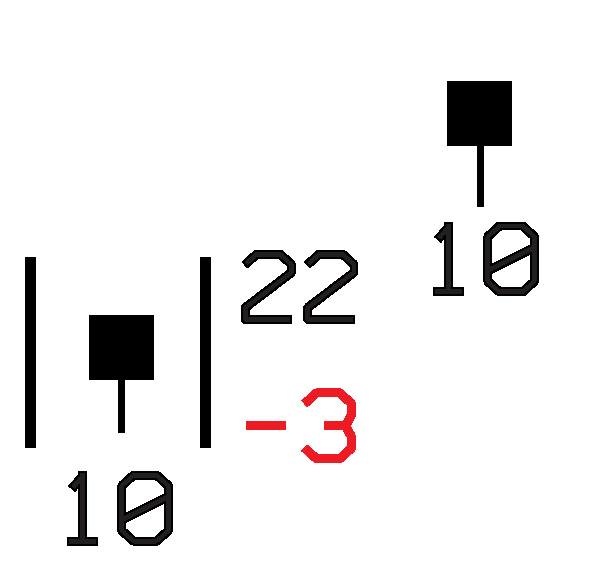
\includegraphics[
                    scale=0.25,
                ]{mfd/fcr_aa/rws_sam_dtt_subfig_01.pdf}
            };
            \node[boxedmarfigstyle] (sam) at (0,-35) {
                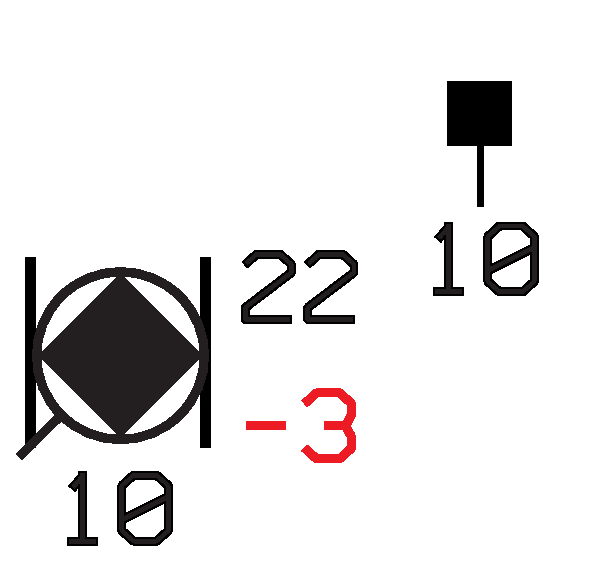
\includegraphics[
                    scale=0.25,
                ]{mfd/fcr_aa/rws_sam_dtt_subfig_02.pdf}
            };

            \draw[->]
            (search) -- node[right, align=center, font=\small] {\textbf{TMS} \textbf{FWD}}(sam);
        \end{tikzpicture}
        \caption{Bugged/STT Symbology}
        % TODO: improve figure
    }%
    For demonstration we will use \textbf{CRM-RWS Submode} 

    \begin{enumerate}
        \item \textbf{Target} \dotfill under \textbf{Acquisition cursor}
        \item \textbf{TMS} \dotfill \textbf{Forward}
        \item \textbf{Target} \dotfill verify \textbf{Bugged}
    \end{enumerate}
    
    If desired can STT lock bugged target

    \begin{enumerate}[start=4]
        \item \textbf{TMS} \dotfill \textbf{Forward}
        \item \textbf{Target} \dotfill verify \textbf{Locked}
    \end{enumerate}
    \blueitem[LOS IFF]
    % \marginpar{
    %     \captionsetup{type=figure}
    %     \fbox{
    %         \begin{minipage}[t][40mm][t]{\marginparwidth}
    %             \center{\textbf{IFF return}}
    %             \begin{itemize}[leftmargin=1em]
    %                 \item maybe show friendly IFF return?
    %             \end{itemize}
    %         \end{minipage}
    %     }
    %     \caption{IFF return, do not shoot!}
    % }%
    % TODO: add iff figure!
    \textbf{See \Cref{sec:iff}}

    \begin{enumerate}
        \item \textbf{TMS} \dotfill \textbf{Left (long)}
        \item \textbf{IFF Returns} \dotfill \textbf{None} (near target)
        \item \textbf{NCTR ID} \dotfill \textbf{Hostile} (if available)
    \end{enumerate}
    \blueitem[Fire Missile]
    \marginpar{
        \captionsetup{type=figure}
        \begin{tikzpicture}[figstyle]
            \node[boxedmarfigstyle] (fig) at (0,0) {
                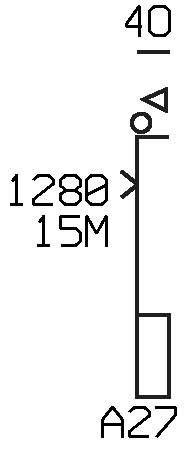
\includegraphics[
                    scale=0.5,
                ]{mfd/fcr_aa/aim120_subfig_dlz_prelaunch.pdf}
            };
        \end{tikzpicture}
        \caption{In-range DLZ}
    }
    \begin{enumerate}
        \item \textbf{ASC} \dotfill within \textbf{ASEC}
        \item \textbf{DLZ} \dotfill indicates \textbf{In-Range}
        \item \textbf{WPN REL} \dotfill \textbf{Depress}
    \end{enumerate}
\end{checklistenumerate}

\clearpage

\subsubsection{MULTI-TARGET EMPLOYMENT}
\label{subsec:aim120:multi}

\begin{checklistenumerate}
    \blueitem[Prerequisites]
    \begin{itemize}
        \item \textbf{FCR Switch} \dotfill \textbf{FCR}
        \item \textbf{Desired MFD} \dotfill \textbf{FCR Page (SOI)}
        \item \textbf{RF Switch} \dotfill \textbf{NORM}
        \item \textbf{Selected Weapon} \dotfill \textbf{120C}
        \item \textbf{SLAVE/BORE} \dotfill Verify \textbf{SLAVE}
        \item \textbf{Master Arm} \dotfill \textbf{ARM}
    \end{itemize}
    \blueitem[CRM Submode] \textbf{As Desired}
    \begin{itemize}
        \item \textbf{RWS} --- max 2-target engagement (DTT) \\
        \textbf{See \Cref{subsec:rws}}
        \item \textbf{TWS} --- true multi-target capability \\
        \textbf{See \Cref{subsec:tws}}
    \end{itemize}
    \blueitem[Track Acquisition]
    For demonstration we will use \textbf{CRM-TWS Submode} 
    \marginpar{
        \captionsetup{type=figure}
        \begin{tikzpicture}[figstyle]

            \node[
                boxedmarfigstyle,            
            ] (track) at (0,0) {
                
\includegraphics[
                    scale=0.5,
                ]{mfd/fcr_aa/tgt_track.pdf}
            };
            \node[
                boxedmarfigstyle,
                below=17.5 of track,
            ] (system) {
                
\includegraphics[
                    scale=0.5,
                ]{mfd/fcr_aa/tgt_system.pdf}
            };
            \node[
                boxedmarfigstyle,                
                below=12.5 of system,
            ] (cursor) {
                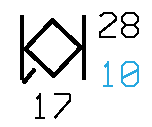
\includegraphics[
                    scale=0.5,
                ]{mfd/fcr_aa/tgt_cursor.pdf}
            };
            \node[
                boxedmarfigstyle,                
                below=10 of cursor,
            ] (bugged) {
                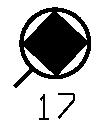
\includegraphics[
                    scale=0.5,
                ]{mfd/fcr_aa/tgt_bugged.pdf}
            };
            \node[
                boxedmarfigstyle,                
                below=10 of bugged,
            ] (dlz) {
                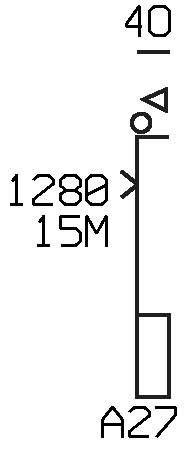
\includegraphics[
                    scale=0.5,
                ]{mfd/fcr_aa/aim120_subfig_dlz_prelaunch.pdf}
            };
            \node[
                boxedmarfigstyle,                
                below=10 of dlz,
            ] (post) {
                
\includegraphics[
                    scale=0.5,
                ]{mfd/fcr_aa/tgt_tail.pdf}
            };

            % lines
            \draw[->]
            (track) -- node[right, align=left, font=\small] {\textbf{TMS FWD} \\ \footnotesize\textbf{(repeat for all} \\ \footnotesize\textbf{desired targets)}}(system);
            \draw[>-]
            ($(track.south)!0.5!(system.north) + (-5,0)$) -- ++(0,2) arc (180:0:2.5) -- ++(0,-4) arc (360:180:2.5) -- node[left, pos=1, align=right, font=\small] {\ref{subsec:aim120:multi:sysacq}} ++(0,2);
            \draw[->]
            (system) -- node[right, align=left, font=\small] {\textbf{Slew Cursor} \\ \textbf{near target}}(cursor);
            \path (system) -- node[left, align=right, font=\small] {\ref{subsec:aim120:multi:acq}}(cursor);
            \draw[->]
            (cursor) -- node[right, align=left, font=\small] {\textbf{TMS FWD}}(bugged);
            \path (cursor) -- node[left, align=right, font=\small] {\ref{subsec:aim120:multi:tmsfwd}}(bugged);
            \draw[->]
            (bugged) -- node[right, align=left, font=\small] {\textbf{In-range}}(dlz);
            \draw[->]
            (dlz) -- node[right, align=left, font=\small] {\textbf{WPN REL}}(post);
            \path (dlz) -- node[left, align=right, font=\small] {\ref{subsec:aim120:multi:wpnrel}}(post);

            % labels
            \node[
                anchor=north west,
                align=left,
                font=\bfseries\footnotesize,
            ] (labeltrack) at (track.north west) {Track \\ Target};
            \node[
                anchor=north west,
                align=left,
                font=\bfseries\footnotesize,
            ] (labelsystem) at (system.north west) {System \\ Target};
            \node[
                anchor=north west,
                align=left,
                font=\bfseries\footnotesize,
            ] (labelcursor) at (cursor.north west) {Cursor \\ Target};
            \node[
                anchor=north west,
                align=left,
                font=\bfseries\footnotesize,
            ] (labelbugged) at (bugged.north west) {Bugged \\ Target};
            \node[
                anchor=north west,
                align=left,
                font=\bfseries\footnotesize,
            ] (labeldlz) at (dlz.north west) {In-Range \\ DLZ};
            \node[
                anchor=north west,
                align=left,
                font=\bfseries\footnotesize,
            ] (labelpost) at (post.north west) {AIM-120 \\ Launched};
        \end{tikzpicture}
        \caption{Multi-target workflow}
    }
    \begin{enumerate}
        \item \textbf{Target} \dotfill under \textbf{Acquisition cursor}
        \item \label{subsec:aim120:multi:sysacq} \textbf{TMS} \dotfill \textbf{Forward}
        \item \textbf{Target} \dotfill verify \textbf{System target}
    \end{enumerate}
    
    Or upgrade \underline{all} tracks to system targets

    \begin{enumerate}
        \item \textbf{TMS} \dotfill \textbf{Right}
    \end{enumerate}
    \blueitem[SCAN IFF]
    \textbf{See \Cref{sec:iff}}

    \begin{enumerate}
        \item \textbf{TMS} \dotfill \textbf{Left (short)}
        \item \textbf{IFF Returns} \dotfill \textbf{None} (near tracks)
    \end{enumerate}
    \blueitem[Bug Acquisition]
    \begin{enumerate}
        \item \label{subsec:aim120:multi:acq}\textbf{Target} \dotfill under \textbf{Acquisition cursor}
        \item \label{subsec:aim120:multi:tmsfwd}\textbf{TMS} \dotfill \textbf{Forward}
        \item \textbf{Target} \dotfill verify \textbf{Bugged}
    \end{enumerate}
    
    Can cycle bugged target with \textbf{TMS Right}
    \blueitem[Fire Missile]
    \begin{enumerate}
        \item \textbf{ASC} \dotfill within \textbf{ASEC}
        \item \textbf{DLZ} \dotfill indicates \textbf{In-Range}
        \item \label{subsec:aim120:multi:wpnrel}\textbf{WPN REL} \dotfill \textbf{Depress}
    \end{enumerate}
    Repeat \crefrange{subsec:aim120:multi:acq}{subsec:aim120:multi:wpnrel} for desired targets
\end{checklistenumerate}

\marginfigrestore

\section[BVR TTP]{BVR TTP --- BEYOND VISUAL RANGE TACTICS, TECHNIQUES, \break AND PROCEDURES}
\label{subsec:bvr}

\subsection[AR FUNDAMENTALS]{ACTIVE RADAR MISSILE FUNDAMENTALS}

\begin{figure}[htbp]
    \centering
    \begin{tikzpicture}[auto, node distance=10mm, x=1mm, y=1mm, very thick, line cap=round,
        >={Latex[round]}
        ]
        % help lines
        % \draw[help lines] (0,-10) grid (100,10);

        % MISSILE
        \coordinate (A_missile) at (0,0);
        \coordinate (B_missile) at (30,10);
        \coordinate (C_missile) at (60,3);
        \coordinate (D_missile) at (80,0);

        \draw[thick, ->]
        (A_missile) .. controls ($(A_missile)+(20,0)$) and ($(B_missile)+(-10,0)$) .. 
        (B_missile) .. controls ($(B_missile)+(5,0)$) and ($(C_missile)+(-10,2.5)$) ..
        (C_missile);
        \draw[dotted, thick, ->] 
        (C_missile) .. controls ($(C_missile)+(10,-2.5)$) and ($(D_missile)+(-5,0)$) ..
        (D_missile);

        \node[above] at (A_missile) {\titlefont A};
        \node[above] at (B_missile) {\titlefont B};
        \node[above] at (C_missile) {\titlefont C};
        \node[above] at (D_missile) {\titlefont D};

        % FIGHTER
        \coordinate (A_fighter) at (A_missile);
        \coordinate (C_fighter) at ($(A_fighter)+(20,0)$);
        \coordinate (D_fighter) at ($(C_fighter)+(-5,-5)$);

        \node[
            anchor=east,
        ] (fig_A_fighter) at (A_fighter) {
            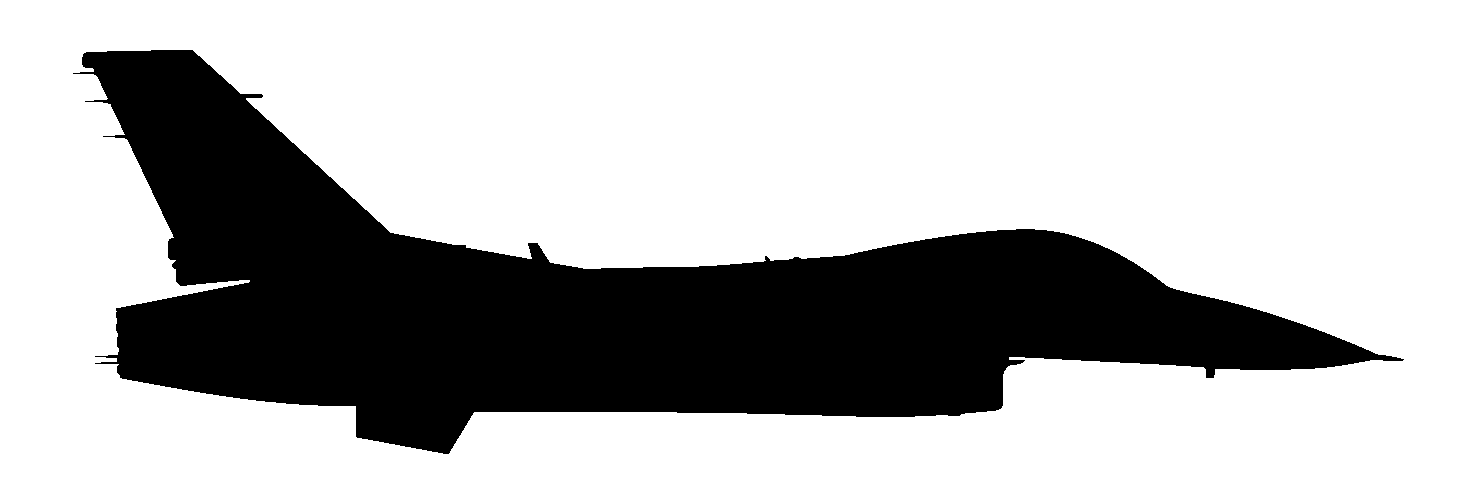
\includegraphics[
                width=7.5mm,
            ]{diagrams/aircraft/silhouette_f16_side.pdf}
        };

        \draw[ultra thick, ->] 
        (A_fighter) -- 
        (C_fighter) .. controls ($(C_fighter)+(5,0)$) and ($(C_fighter)+(5,-5)$) .. 
        ($(C_fighter)+(0,-5)$) --
        (D_fighter);

        \node[above right] at (C_fighter) {\titlefont C};
        \node[left] at (D_fighter) {\titlefont D};

        % BANDIT
        \coordinate (A_bandit) at (100,0);
        \coordinate (C_bandit) at (85,0);
        \coordinate (D_bandit) at (D_missile);

        \draw[ultra thick, ->] 
        (A_bandit) -- 
        (D_bandit);

        \node[above] at (A_bandit) {\titlefont A};
        \node[above] at (C_bandit) {\titlefont C};

        \filldraw[red] (D_bandit) circle (2pt);

        % Distance lines
        \draw[thin, <->]
        ($(C_fighter)+(0,-12.5)$) -- node[pos=0.5, above]{\small\titlefont R\textsubscript{A-POLE}}
        ($(C_bandit)+(0,-12.5)$);
        \draw[thin, <->]
        (15,-20) -- node[pos=0.5, above]{\small\titlefont R\textsubscript{F-POLE}}
        ($(D_missile)+(0,-20)$);
        \draw[thin, <->]
        ($(A_missile)+(0,-27.5)$) -- node[pos=0.5, above]{\small\titlefont R\textsubscript{LAUNCH}}
        ($(A_bandit)+(0,-27.5)$);

        \draw[thin]
        ($(C_fighter)+(0,-2.5)$) -- ($(C_fighter)+(0,-15)$)
        ($(C_bandit)+(0,-2.5)$) -- ($(C_bandit)+(0,-15)$)
        ($(D_fighter)+(0,-2.5)$) -- (15,-22.5)
        ($(D_missile)+(0,-2.5)$) -- ($(D_missile)+(0,-22.5)$)
        ($(A_missile)+(0,-2.5)$) -- ($(A_missile)+(0,-30)$)
        ($(A_bandit)+(0,-2.5)$) -- ($(A_bandit)+(0,-30)$);

    \end{tikzpicture}
    \caption{Side-on view of a generic AIM-120 employment profile}
    \label{fig:aa_weap:bvr:aim120profile}
    % TODO: silhouettes?
\end{figure}

\begin{tcoloritemize}
    \blueitem{AIM-120 \break Employment \break Profile}{
    \Cref{fig:aa_weap:bvr:aim120profile} shows the trajectories of fighter, bandit \& missile for a generic AIM-120 employment profile
    including the following phases

    \begin{itemize}
        \item \textbf{A --- Launch / Boost Phase}
        \item \textbf{B --- Mid-Course Phase}
        \item \textbf{C --- Acquisition}
        \item \textbf{D --- Intercept}
    \end{itemize}}
    \blueitem{Launch / Boost Phase}{
    \textbf{Boost}

    \begin{itemize}
        \item Motor only fires for initial seconds of flight 
        \item After burnout missile \textbf{\underline{cannot gain energy}}
    \end{itemize}

    \textbf{Lofting} 

    \begin{itemize}
        \item To reach longer ranges missile ``lofts'' itself to conserve energy \& optimize trajectory
        \item Pilot can manually loft by raising the nose 20-30 deg prior to launch
    \end{itemize}
    }
    \blueitem{Mid-Course Phase}{
    \textbf{Missile flies using internal IMU}

    \begin{itemize}
        \item Receives periodic datalink updates
        \item Will fly to last updated target position if DL lost
    \end{itemize}}
    \blueitem{Acquisition \& MPRF ``Active'' Phase}{
    \textbf{Missile radar turns on once close to target location}
    \begin{itemize}
        \item Seeker in MPRF (Medium Pulse Repetition Frequency) mode 
        \item Locks on to closest / best target
    \end{itemize}}
    \blueitem{Terminal Phase \& Intercept}{
    \textbf{Once missile seeker has acquired target}
    \begin{itemize}
        \item Flies PNG intercept trajectory
        \item Requires no further DL support, fighter can turn away from the bandit
    \end{itemize}}
\end{tcoloritemize}

\warningbox{
    \textbf{AIM-120 HAS \underline{NO} IFF FUNCTIONALITY} --- use caution near friendlies
}

\subsubsection{TACTICAL CONSIDERATIONS}
\label{subsec:bvr:tacticalconsideration}
% \label{subsec:aim120:tactics}
\begin{tcoloritemize}
    \blueitem{Range Definitions}{
    \textbf{Fighter-bandit distance} can be measured at different points during the timeline

    \begin{itemize}
        \item \textbf{R\textsubscript{Launch}} --- distance at launch
        \item \textbf{R\textsubscript{A-Pole}} --- distance when missile goes active
        \item \textbf{R\textsubscript{F-Pole}} --- distance at impact
    \end{itemize}
    
    These are also illustrated in \cref{fig:aa_weap:bvr:aim120profile}.
    }
    \blueitem{Maximizing Launch Range / Energy}{
    \textbf{Why?}
    \begin{itemize}
        \item Ability to launch at longer ranges forces bandit defensive
        \item Bandit may not be able to counter-launch
        \item Higher launch energy increases P\textsubscript{intercept} %probability of intercept
    \end{itemize}
    \textbf{How?}
    \begin{itemize}
        \item \textbf{High velocity} --- increases kinetic energy 
        \item \textbf{High altitude} --- increases potential energy, reduces drag
    \end{itemize}}
    \blueitem{Maximizing \break F-Pole Range}{
    \textbf{Why?}
    \begin{itemize}
        \item Less likely to enter bandit launch envelope
        \item More time/range to launch 2nd missile if necessary
    \end{itemize}
    \textbf{How?}
    \begin{itemize}
        \item \textbf{Crank} --- turn 45-60 degrees away from bandit to reduce closure rate, maintain radar contact
        \item \textbf{Dive} --- reduces threat missile envelope
    \end{itemize}}
    \blueitem{Flowing Cold}{
    \textbf{Why?}
    \begin{itemize}
        \item Missile requires no support once active
        \item Defend against unknown missile launches
        \item Maximize F-pole range further
    \end{itemize}
    \textbf{How?}
    \begin{itemize}
        \item \textbf{Turn} --- Away from bandit / threat
        \item \textbf{Dive} --- if necessary, reduces threat missile envelope 
    \end{itemize}}
    \blueitem{Effect of Bandit Maneuvers}{
    As evident in \cref{fig:aa_weap:bvr:aim120profile}, 
   \textbf{R\textsubscript{Launch}} is significantly greater than the distance travelled by the missile
    \begin{itemize}
        \item \textbf{DLZ calculated based off \underline{both} fighter \underline{and} bandit velocity/altitude}
        \item Bandit can significantly change missile envelope by reducing closure rate / altitude
        \item Post-launch bandit maneuvers can result in missile not having energy to intercept
    \end{itemize}}
\end{tcoloritemize}

\clearpage

\subsubsection{FIGHTER MANEUVERS}

\begin{tcoloritemize}
    \blueitem{Crank}{Fighter turns \textbf{45-60 deg} away from threat 

    \begin{itemize}
        \item reduces closure while maintaining radar track
        \item typically used post-launch
    \end{itemize}
    
    Reference \cref{fig:aa_weap:bvr:fightermaneuver:crank}
    }
    \blueitem{Notch}{Fighter turns \textbf{70-110 deg} away from threat

    \begin{itemize}
        \item minimizes relative velocity to break hostile pulse-doppler radar track
        \item increases angular motion, forcing missile to maneuver and expend energy
    \end{itemize}
    
    Reference \cref{fig:aa_weap:bvr:fightermaneuver:notch}
    }
    \blueitem{Go Cold}{Fighter turns \textbf{away} from threat

    \begin{itemize}
        \item used to kinematically defeat threat missiles
    \end{itemize}
    
    Reference \cref{fig:aa_weap:bvr:fightermaneuver:cold}}
\end{tcoloritemize}

\begin{figure}[htbp]
    \centering
    \begin{subfigure}[b]{0.3\linewidth}
        \centering
        \begin{tikzpicture}[figstyle]
            % FIGHTER
            \node[
                anchor=north,
                yshift=1mm,
            ] (fighter) at (0,0) {
                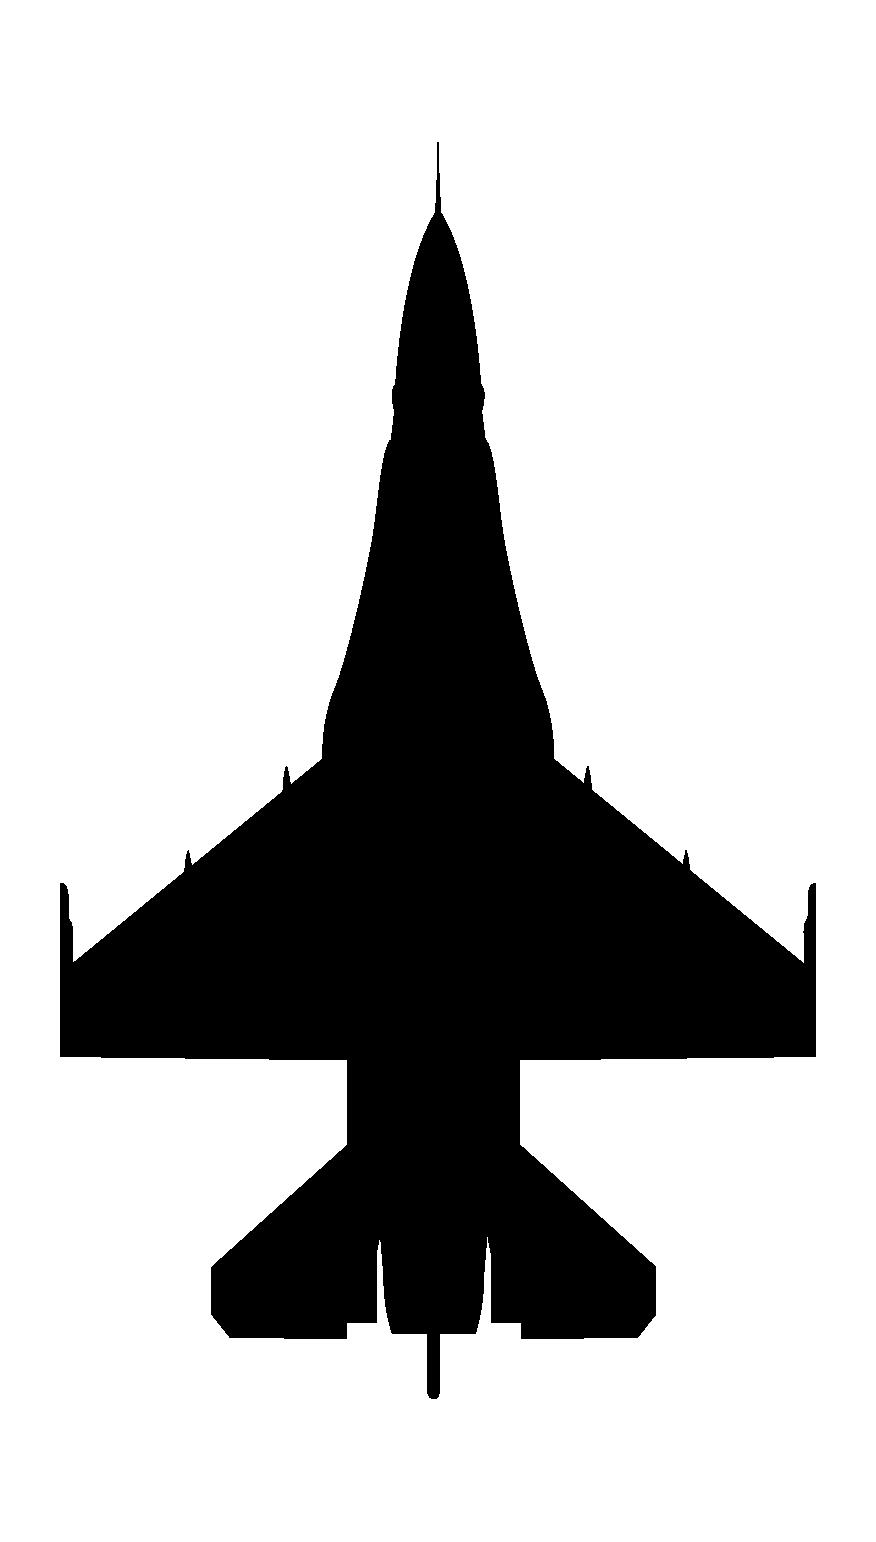
\includegraphics[
                    width=7.5mm,
                ]{diagrams/aircraft/silhouette_f16_top.pdf}
            };
            \draw[very thick, rounded corners, ->] 
            (0,0) -- (0,5) -- +(30:15) node[rotate=-60, anchor=south, yshift=-1mm]{
                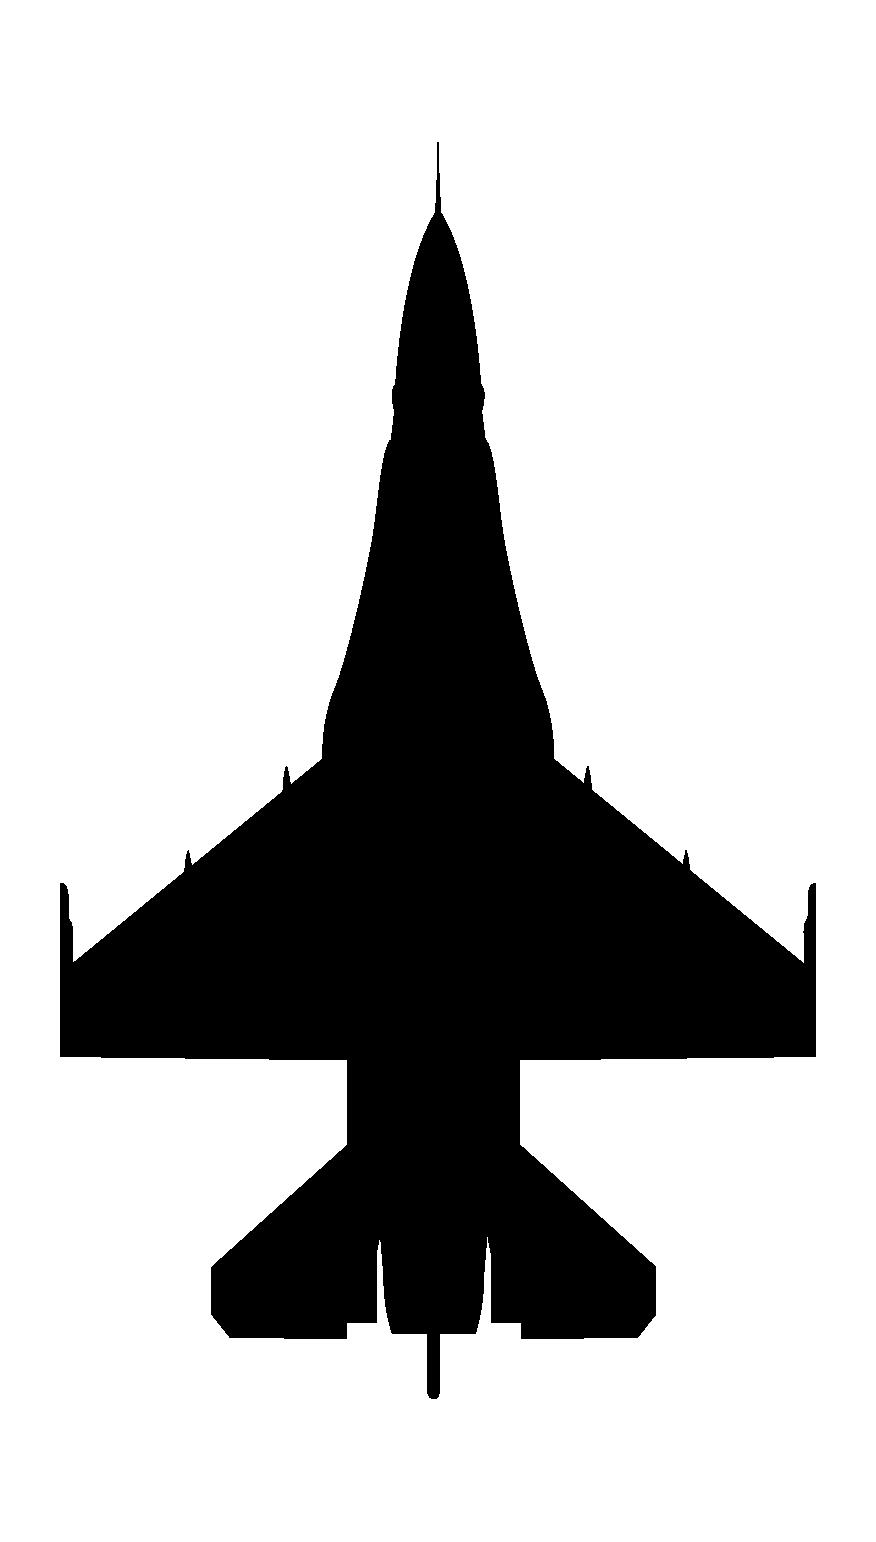
\includegraphics[
                width=7.5mm,
            ]{diagrams/aircraft/silhouette_f16_top.pdf}};
    
            % BANDIT
            \draw[very thick, rounded corners, ->] 
            (0,35) -- (0,25);
    
            % help line
            \draw[thin, dashed] 
            (0,25) -- (0,5);
    
            \draw[thin]
            (0,15) arc (90:30:10) node[pos=0.15, above right]{\small\titlefont 45-60$^\circ$};
    
        \end{tikzpicture}
        \caption{Crank}
        \label{fig:aa_weap:bvr:fightermaneuver:crank}
    \end{subfigure}
    \begin{subfigure}[b]{0.3\linewidth}
        \centering
        \begin{tikzpicture}[figstyle]
            % FIGHTER
            \node[
                anchor=north,
                yshift=1mm,
            ] (fighter) at (0,0) {
                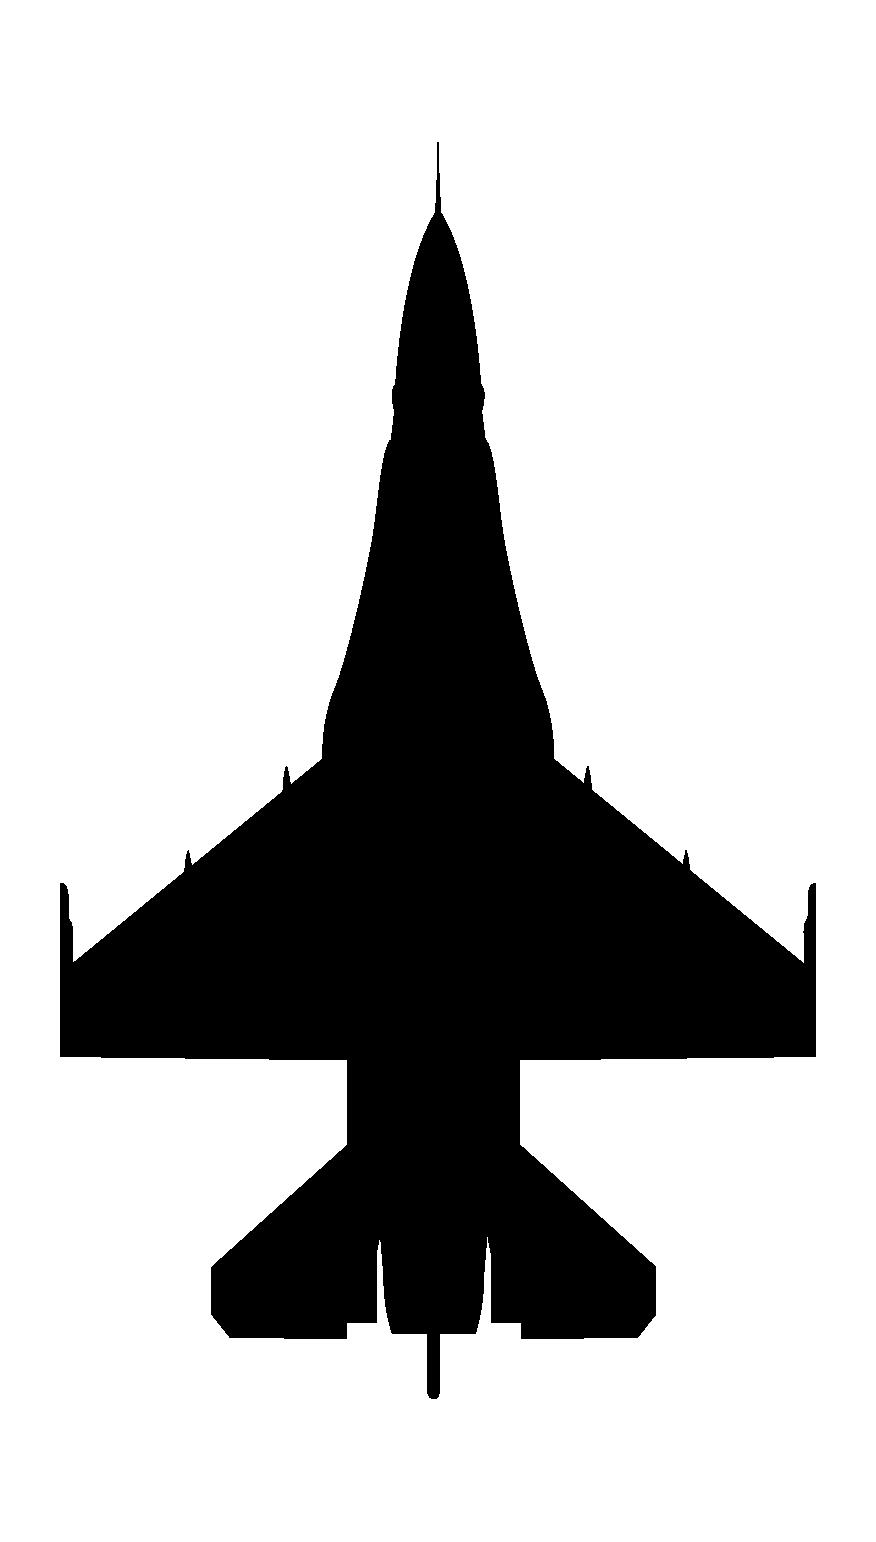
\includegraphics[
                    width=7.5mm,
                ]{diagrams/aircraft/silhouette_f16_top.pdf}
            };
            \draw[very thick, rounded corners, ->] 
            (0,0) -- (0,5) -- +(0:15) node[rotate=-90, anchor=south, yshift=-1mm]{
                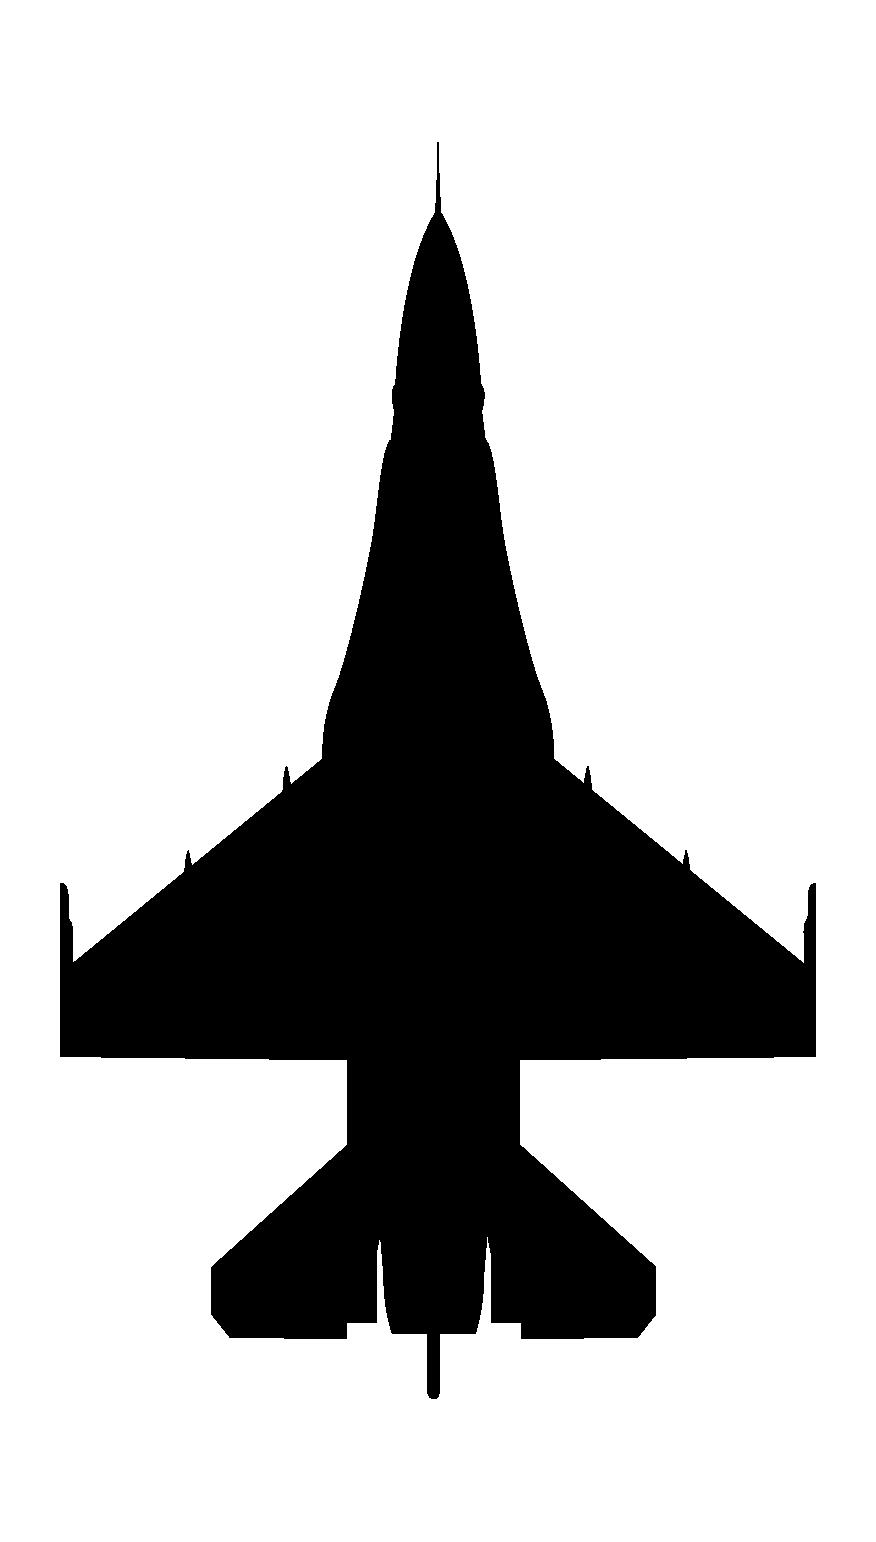
\includegraphics[
                width=7.5mm,
            ]{diagrams/aircraft/silhouette_f16_top.pdf}};
    
            % BANDIT
            \draw[very thick, rounded corners, ->] 
            (0,35) -- (0,25);
    
            % help line
            \draw[thin, dashed] 
            (0,25) -- (0,5);
    
            \draw[thin]
            (0,15) arc (90:0:10) node[pos=0.5, above right]{\small\titlefont 70-110$^\circ$};
    
        \end{tikzpicture}
        \caption{Notch}
        \label{fig:aa_weap:bvr:fightermaneuver:notch}
    \end{subfigure}
    \begin{subfigure}[b]{0.3\linewidth}
        \centering
        \begin{tikzpicture}[figstyle]
            % FIGHTER
            \node[
                anchor=north,
                yshift=1mm,
            ] (fighter) at (0,0) {
                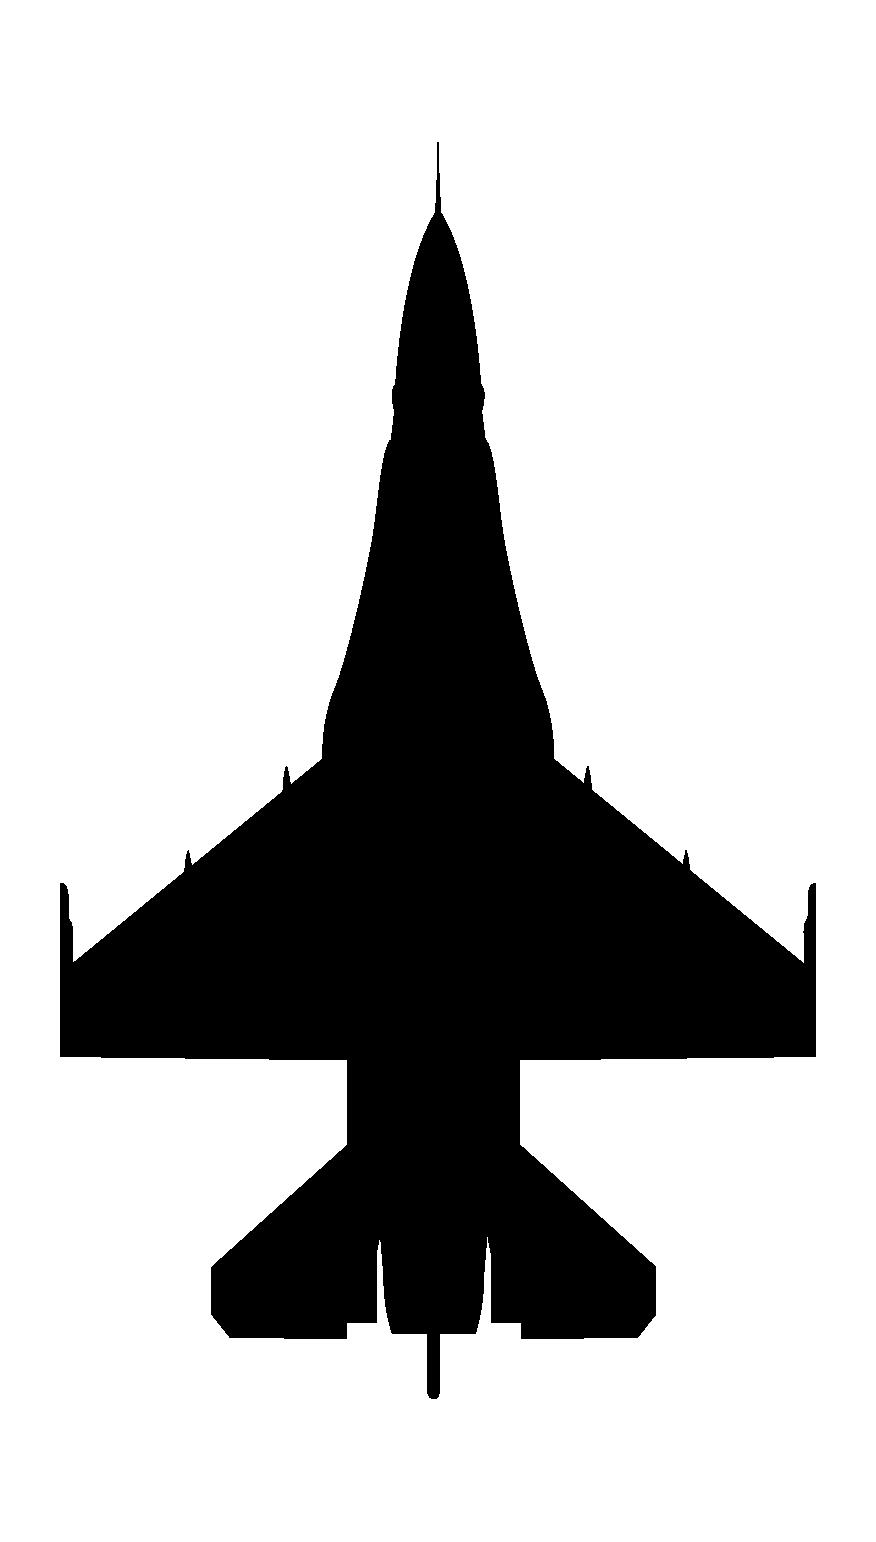
\includegraphics[
                    width=7.5mm,
                ]{diagrams/aircraft/silhouette_f16_top.pdf}
            };
            \draw[very thick, ->] 
            (0,0) -- 
            (0,5) arc (180:0:5) --
            (10,0) 
            node[rotate=-180, anchor=south, yshift=-1mm]{
                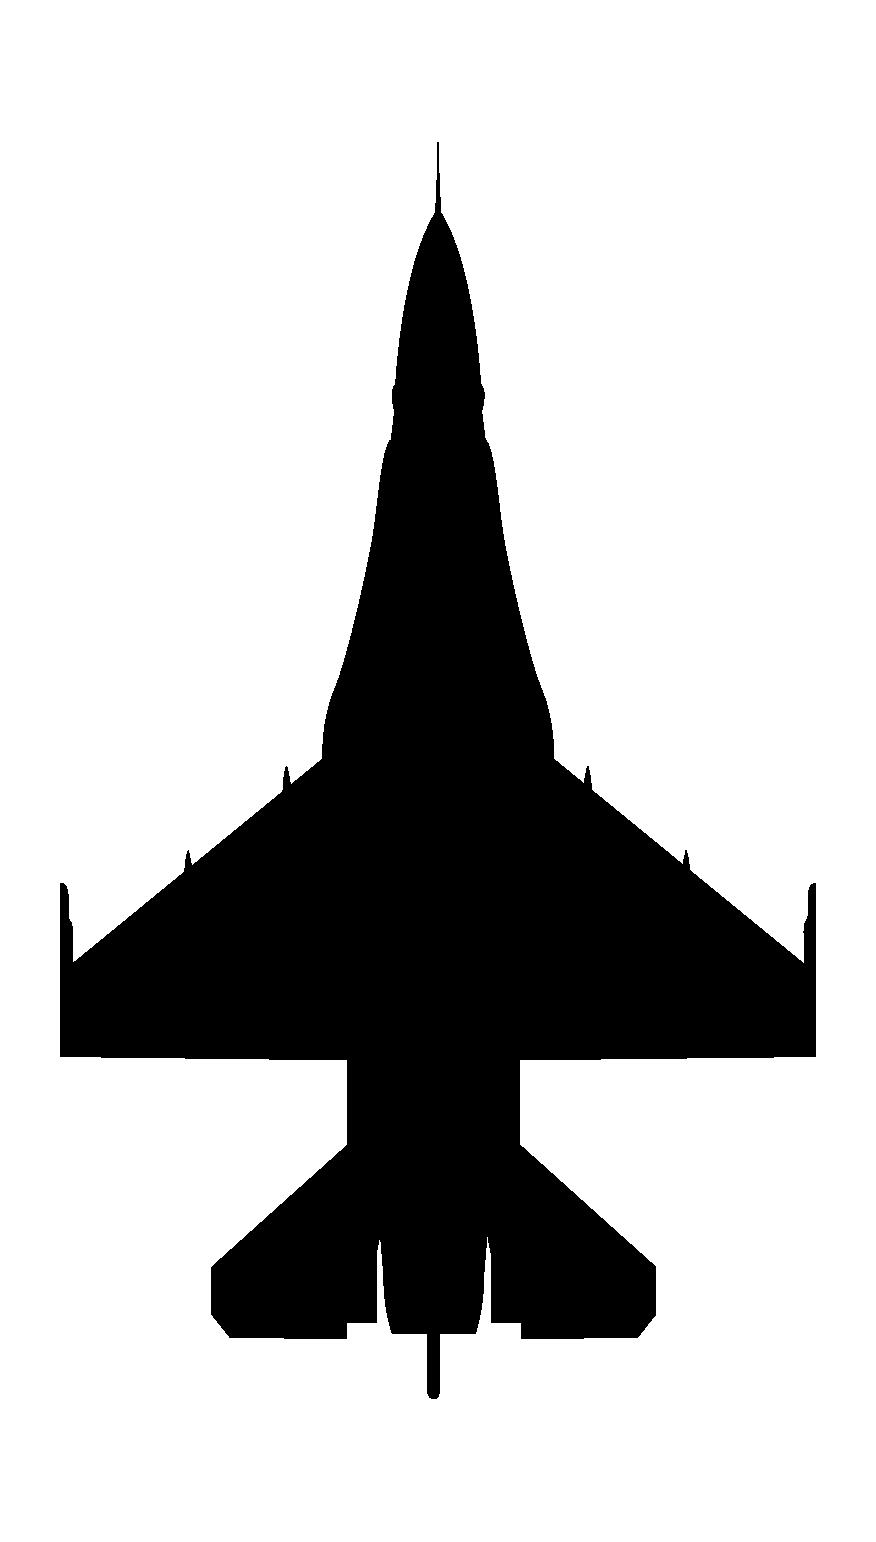
\includegraphics[
                width=7.5mm,
            ]{diagrams/aircraft/silhouette_f16_top.pdf}};
    
            % BANDIT
            \draw[very thick, rounded corners, ->] 
            (0,35) -- (0,25);

            % help line
            \draw[thin, dashed] 
            (0,25) -- (0,5);

        \end{tikzpicture}
        \caption{Go Cold}
        \label{fig:aa_weap:bvr:fightermaneuver:cold}
    \end{subfigure}
    \caption{Top-down view of basic BVR fighter maneuvers}
    \label{fig:aa_weap:bvr:fightermaneuver}
\end{figure}

\warningbox{
    \textbf{Turning in after going cold can place fighter within bandit launch envelope}
}

\subsubsection{TARGET ASPECT}

\begin{tcoloritemize}
    \blueitem{Target Aspect}{Angle between imaginary line connecting fighter-bandit and bandit heading}
    \blueitem{Hot}{\textbf{Target aspect --- 0-40 deg}
    \begin{itemize}
        \item offensive posture, maximizes closure
    \end{itemize}}
    \blueitem{Flank}{\textbf{Target aspect --- 40-70 deg}
    \begin{itemize}
        \item minimizes closure while maintaining radar track
    \end{itemize} }
    \blueitem{Beam}{\textbf{Target aspect --- 70-110 deg}
    \begin{itemize}
        \item defensive maneuver to break pulse-doppler radar track
    \end{itemize}}
    \blueitem{Drag}{\textbf{Target aspect --- 110-180 deg}
    \begin{itemize}
        \item defense to kinematically defeat missile
        \item often used in group tactics as ambush setup
    \end{itemize}}
\end{tcoloritemize}

\begin{figure}[htbp]
    \centering
    \begin{subfigure}[b]{0.2\linewidth}
        \centering
        \begin{tikzpicture}[figstyle]
            % FIGHTER
            \node[
                anchor=north,
                yshift=1mm,
            ] (fighter) at (0,0) {
                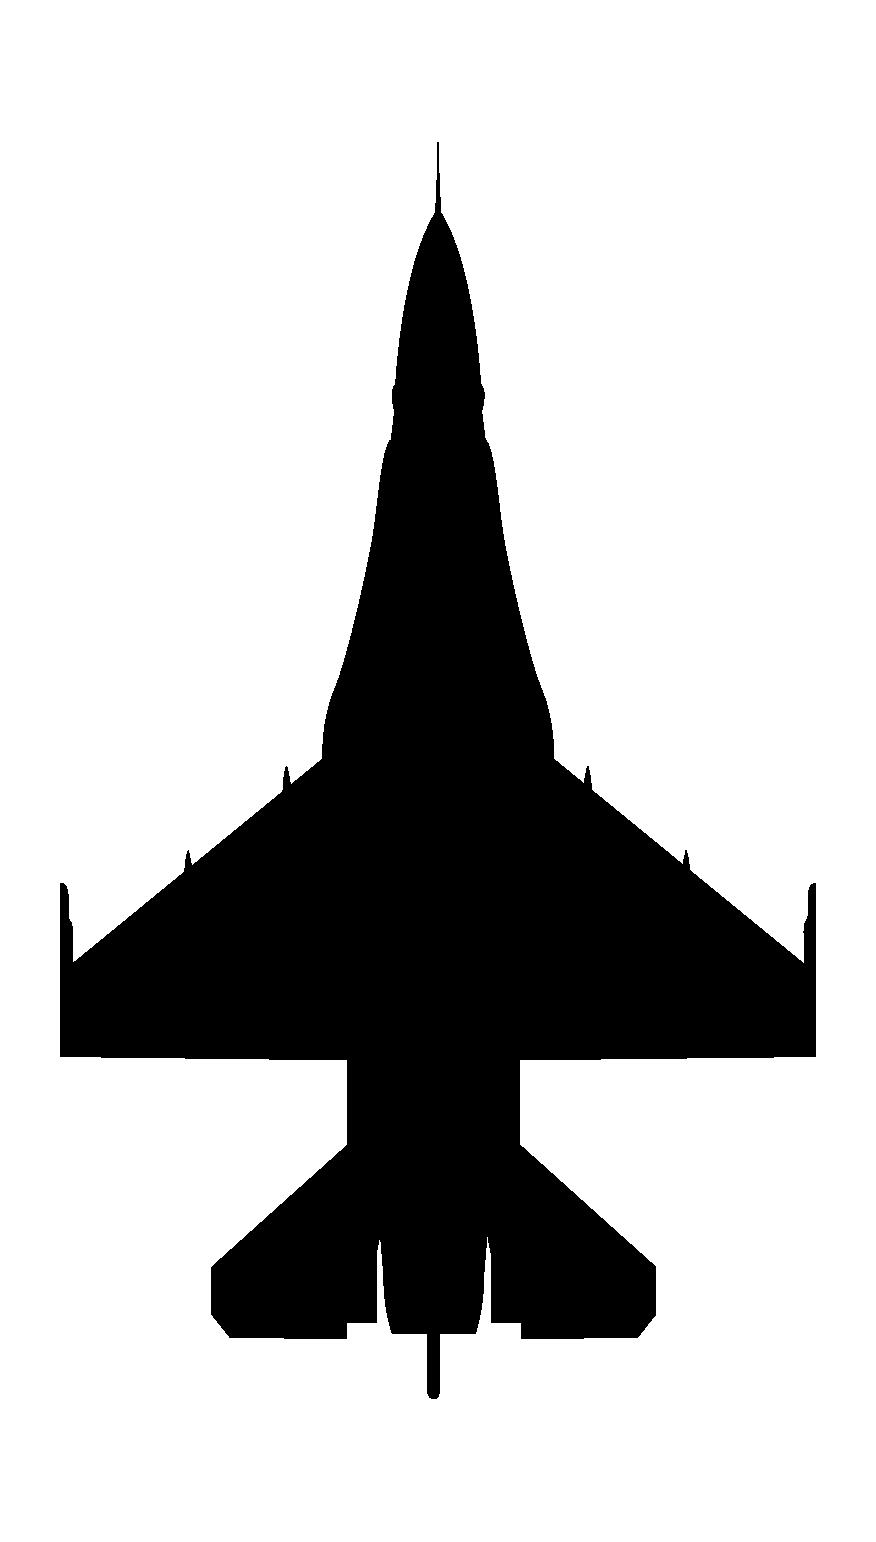
\includegraphics[
                    width=7.5mm,
                ]{diagrams/aircraft/silhouette_f16_top.pdf}
            };
    
            % BANDIT
            \draw[very thick, rounded corners, ->] 
            (0,20) -- +(-75:15);
    
            % help line
            \draw[thin, dashed] 
            (0,20) -- (0,0);
    
            \draw[thin]
            (0,10) arc (-90:-75:10) node[pos=1.0, right]{\small\titlefont 0-40$^\circ$};

        \end{tikzpicture}
        \caption{Hot}
        \label{fig:aa_weap:bvr:ta:hot}
    \end{subfigure}
    \begin{subfigure}[b]{0.2\linewidth}
        \centering
        \begin{tikzpicture}[figstyle]
            % FIGHTER
            \node[
                anchor=north,
                yshift=1mm,
            ] (fighter) at (0,0) {
                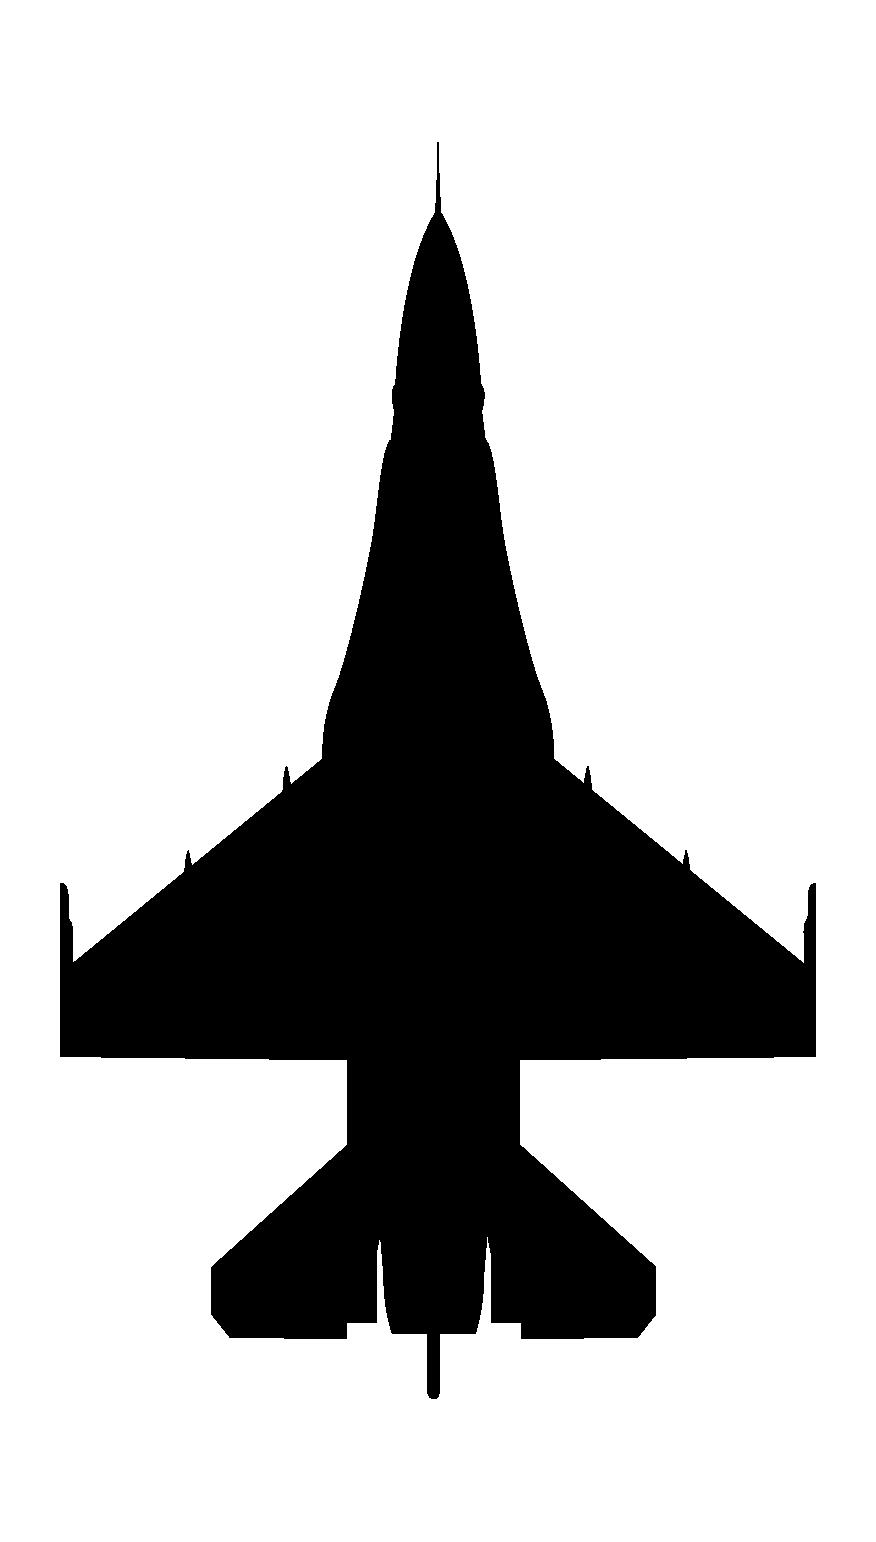
\includegraphics[
                    width=7.5mm,
                ]{diagrams/aircraft/silhouette_f16_top.pdf}
            };
    
            % BANDIT
            \draw[very thick, rounded corners, ->] 
            (0,20) -- +(-30:15);
    
            % help line
            \draw[thin, dashed] 
            (0,20) -- (0,0);
    
            \draw[thin]
            (0,10) arc (-90:-30:10) node[pos=0.25, below right]{\small\titlefont 40-70$^\circ$};

        \end{tikzpicture}
        \caption{Flank}
        \label{fig:aa_weap:bvr:ta:flank}
    \end{subfigure}
    \begin{subfigure}[b]{0.25\linewidth}
        \centering
        \begin{tikzpicture}[figstyle]
            % FIGHTER
            \node[
                anchor=north,
                yshift=1mm,
            ] (fighter) at (0,0) {
                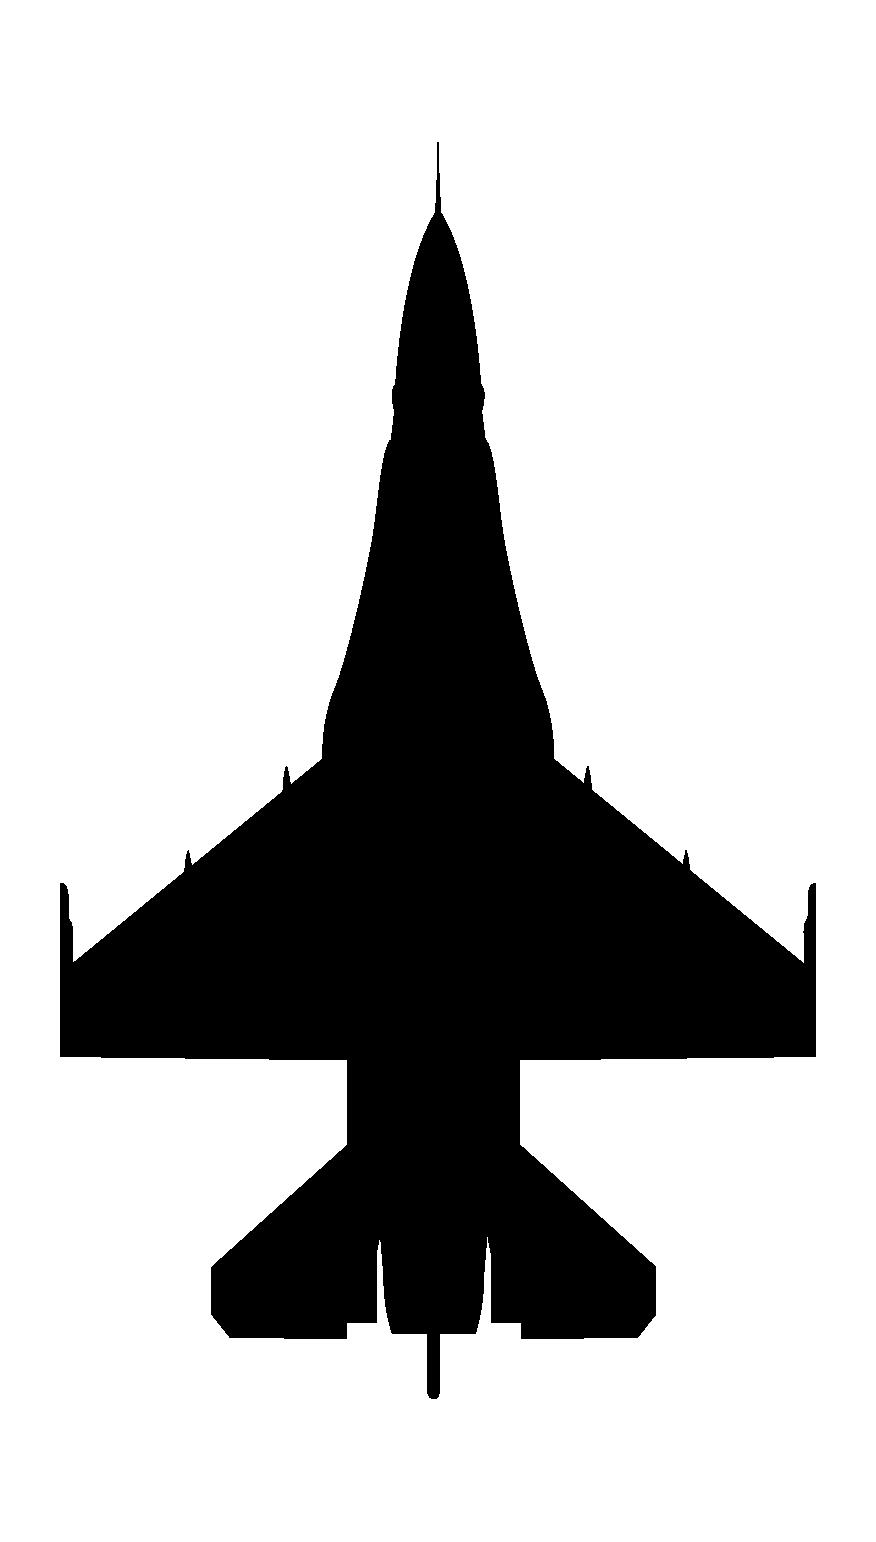
\includegraphics[
                    width=7.5mm,
                ]{diagrams/aircraft/silhouette_f16_top.pdf}
            };
    
            % BANDIT
            \draw[very thick, rounded corners, ->] 
            (0,20) -- +(0:15);
    
            % help line
            \draw[thin, dashed] 
            (0,20) -- (0,0);
    
            \draw[thin]
            (0,10) arc (-90:0:10) node[pos=0.25, below right]{\small\titlefont 70-110$^\circ$};
    
        \end{tikzpicture}
        \caption{Beam}
        \label{fig:aa_weap:bvr:ta:beam}
    \end{subfigure}
    \begin{subfigure}[b]{0.25\linewidth}
        \centering
        \begin{tikzpicture}[figstyle]
            % FIGHTER
            \node[
                anchor=north,
                yshift=1mm,
            ] (fighter) at (0,0) {
                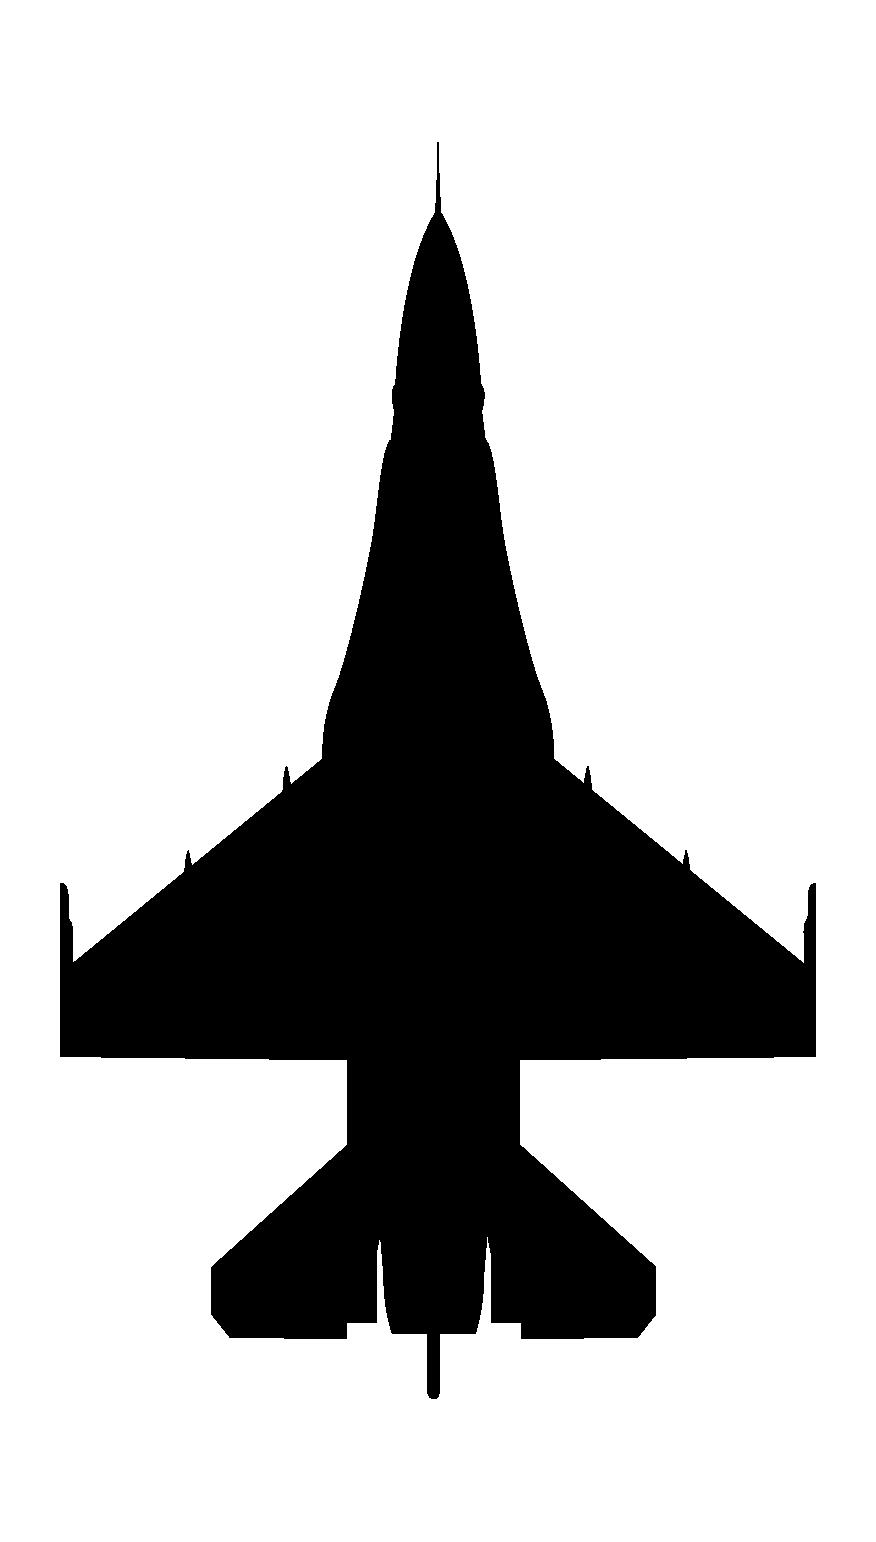
\includegraphics[
                    width=7.5mm,
                ]{diagrams/aircraft/silhouette_f16_top.pdf}
            };
    
            % BANDIT
            \draw[very thick, rounded corners, ->] 
            (0,20) -- +(90:15);
    
            % help line
            \draw[thin, dashed] 
            (0,20) -- (0,0);
    
            \draw[thin]
            (0,10) arc (-90:90:10) node[pos=0.125, below right]{\small\titlefont 110-180$^\circ$};
    
        \end{tikzpicture}
        \caption{Drag}
        \label{fig:aa_weap:bvr:ta:drag}
    \end{subfigure}
    \caption{Top down view illustrating target aspect classification}
    \label{fig:aa_weap:bvr:ta}
\end{figure}

\marginfigeometry

\subsection{INTERCEPT TIMELINES}

% \subsubsection{SKATE}
% \subsubsection{SHORT SKATE}
% \subsubsection{BANZAI}

\marginpar{
    \captionsetup{type=figure}
    \centering
    \begin{tikzpicture}[figstyle]
        
        \draw[very thick, ->] 
            (0,0) -- 
            node[below, pos=0]{
                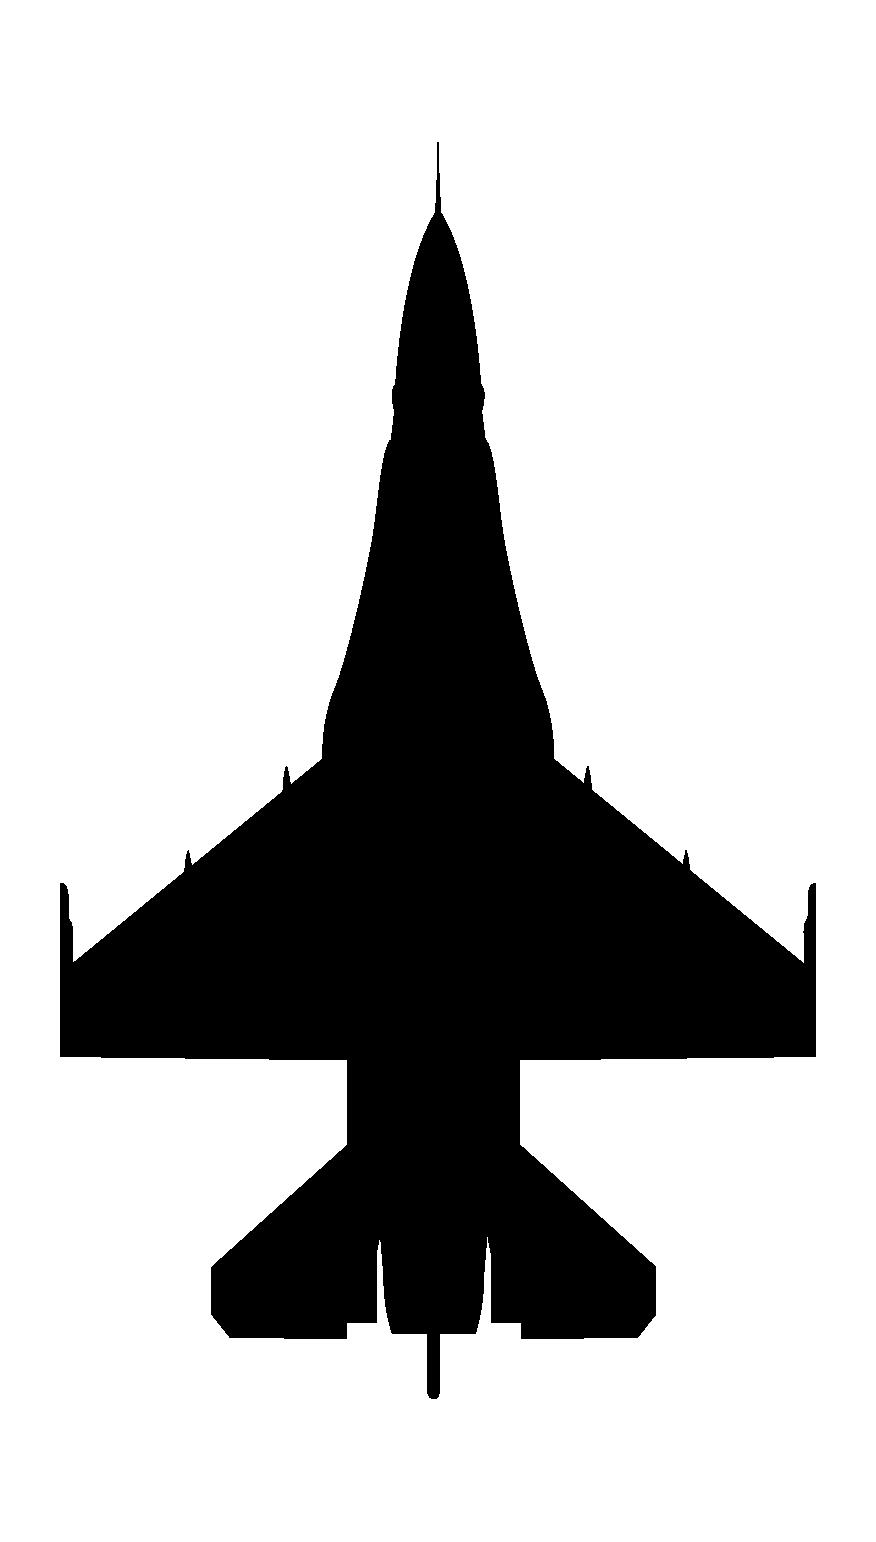
\includegraphics[
                width=7.5mm,
            ]{diagrams/aircraft/silhouette_f16_top.pdf}} 
            ++(0,20) 
            arc (180:90:5) 
            arc (-90:0:5) 
            -- ++(0,20) 
            arc (180:0:5) 
            -- ++(0,-50)
            node[below, pos=1, ]{
                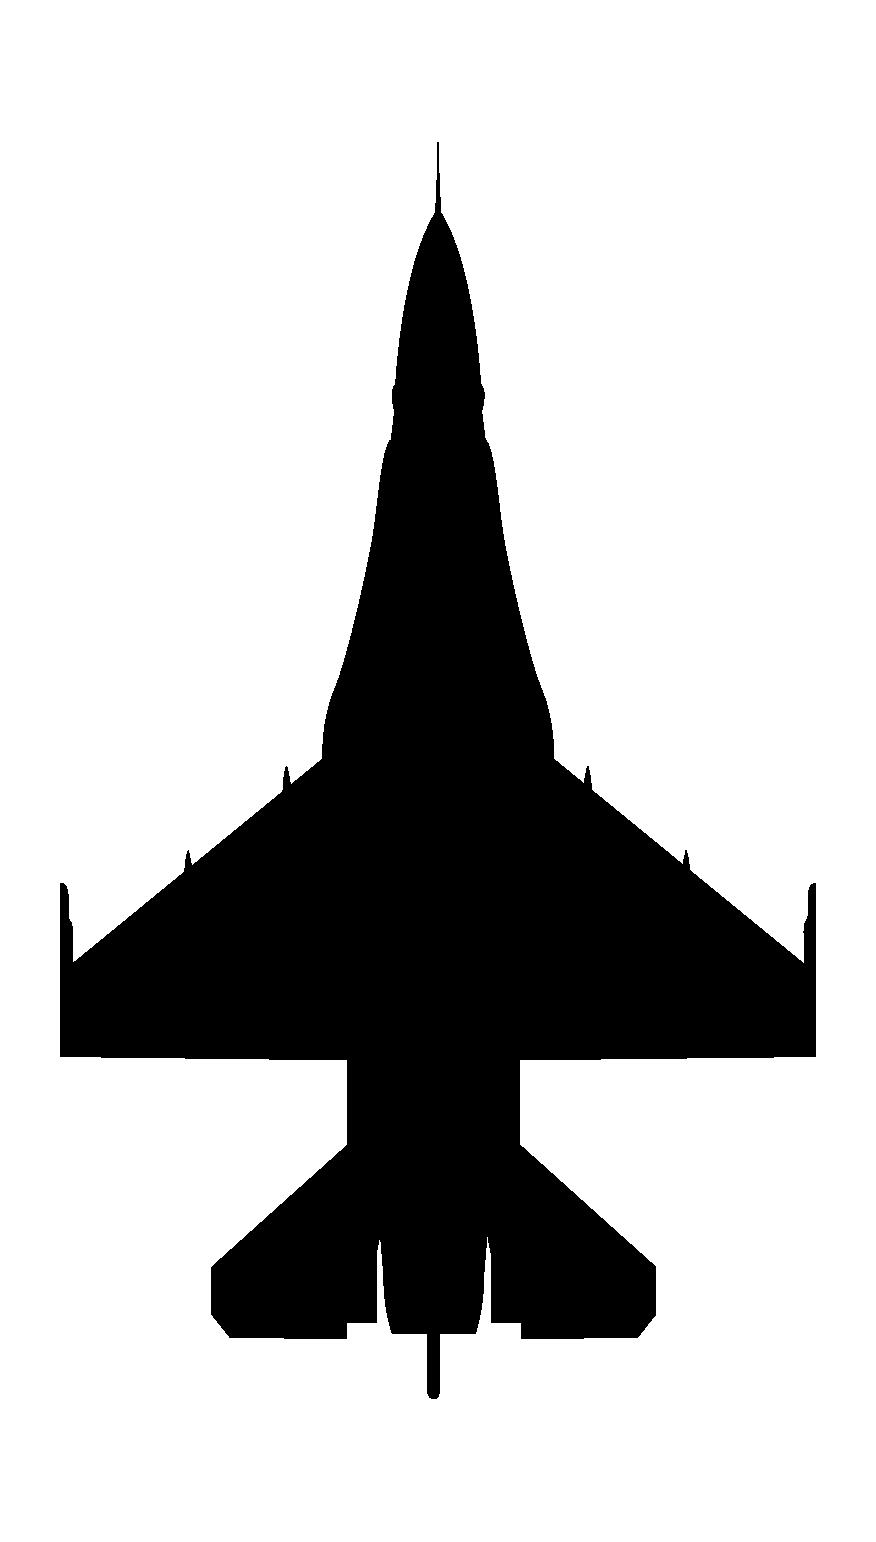
\includegraphics[
                    angle=180,
                    width=7.5mm,
            ]{diagrams/aircraft/silhouette_f16_top.pdf}};

    \end{tikzpicture}
    \caption{Work in progress timeline illustration}
}
\begin{center}
    \vspace{\textheight/4}
    \Large\titlefont\textbf{COMING SOON}
\end{center}

\marginfigrestore